% ============================================================
% A Coupled Power-Thermal-Cyber Framework for Actuarial Pricing
% and Insurance of Hyperscale Data Centers
%
% Working paper - novel framework integrating electrical
% reliability engineering, mathematical statistics, and
% actuarial mathematics.
%
% Visual theme: institutional research house — deep warm black,
% bone background, burnt-sienna accent rules. Palatino serif body,
% Helvetica sans headings.
% ============================================================
\documentclass[11pt,a4paper]{article}

% --- math ---
\usepackage{amsmath,amssymb,amsthm,mathtools,bm}
\usepackage{siunitx}
\sisetup{detect-all,group-separator={,},per-mode=symbol}

% --- layout ---
\usepackage[a4paper,margin=1in,headheight=14pt,headsep=18pt]{geometry}
\usepackage{booktabs,array,tabularx,multirow}
\usepackage[T1]{fontenc}
\usepackage{enumitem}
\usepackage{xcolor}
\usepackage{tcolorbox}
\tcbuselibrary{breakable,skins}

% --- typography: Palatino serif body + Helvetica sans, matching math
% This is the standard institutional-research-house combination.
\usepackage{mathpazo}
\linespread{1.08}             % a touch more leading for premium feel
\usepackage[scaled=0.92]{helvet}  % sans family, slightly scaled
\usepackage{courier}              % monospace
\usepackage{microtype}            % subtle horizontal balance

% --- IA brand colour palette ---
% deep warm near-black (signature dark from intelligentactuaries.com)
\definecolor{iadark}{HTML}{1B1815}
% bone / cream paper background
\definecolor{iabone}{HTML}{FAFAF7}
% burnt sienna accent (institutional warmth)
\definecolor{iaaccent}{HTML}{A04A1F}
% soft taupe / pale background for callouts
\definecolor{iataupe}{HTML}{F2EDE6}
% subtle rule colour
\definecolor{iarule}{HTML}{3A332D}
% supporting grey for captions
\definecolor{iagrey}{HTML}{5A524A}

% Apply the bone background to the page
\pagecolor{iabone}

% --- graphics ---
\usepackage{tikz}
\usepackage{circuitikz}
\usepackage{pgfplots}
\pgfplotsset{compat=1.18}
\usetikzlibrary{arrows.meta,positioning,shapes.geometric,calc,fit,
                decorations.pathreplacing,decorations.markings,
                shadows.blur,backgrounds}

% --- algorithms & refs ---
\usepackage{algorithm}
\usepackage{algpseudocode}
\usepackage[numbers,sort&compress]{natbib}
\usepackage[colorlinks=true,linkcolor=iaaccent,citecolor=iaaccent,
            urlcolor=iaaccent]{hyperref}

% --- section title styling (titlesec) ---
\usepackage{titlesec}
% Numbered sections: sans bold, IA dark, accent rule underneath
\titleformat{\section}
  {\sffamily\bfseries\large\color{iadark}}
  {\thesection.}{0.6em}
  {}
  [\vspace{2pt}{\color{iaaccent}\titlerule[0.6pt]}]
\titleformat{\subsection}
  {\sffamily\bfseries\normalsize\color{iadark}}
  {\thesubsection.}{0.5em}
  {}
\titleformat{\subsubsection}
  {\sffamily\bfseries\small\color{iadark}}
  {\thesubsubsection.}{0.5em}
  {}
\titlespacing*{\section}{0pt}{14pt}{6pt}
\titlespacing*{\subsection}{0pt}{10pt}{4pt}
\titlespacing*{\subsubsection}{0pt}{8pt}{3pt}

% --- caption styling ---
\usepackage[font={small,sf},labelfont={bf,color=iadark},
            textfont={color=iagrey},labelsep=colon]{caption}

% --- running headers/footers ---
\usepackage{fancyhdr}
\pagestyle{fancy}
\fancyhf{}
\renewcommand{\headrulewidth}{0pt}
\renewcommand{\footrulewidth}{0pt}
% header: title on left, section/chapter on right, hairline rule underneath
\fancyhead[L]{\footnotesize\sffamily\color{iagrey}%
  Coupled Power--Thermal--Cyber Framework}
\fancyhead[R]{\footnotesize\sffamily\color{iagrey}\nouppercase{\leftmark}}
\fancyfoot[C]{\footnotesize\sffamily\color{iadark}\thepage}
\renewcommand{\sectionmark}[1]{\markboth{\thesection\quad #1}{}}
\addtolength{\headheight}{2pt}
% draw the accent hairline rule under the header
\AtBeginDocument{\renewcommand{\headrule}{%
  {\color{iaaccent}\hrule height 0.4pt}\vspace{1pt}%
  {\color{iarule}\hrule height 0.15pt}}}
\renewcommand{\headrulewidth}{0.4pt}

% --- theorem styles, with IA-style accent ---
\newtheoremstyle{ia}
  {6pt}{6pt}              % above/below
  {\itshape}              % body font
  {0pt}                   % indent
  {\sffamily\bfseries\color{iadark}}    % head font
  {.}                     % head punct
  {.6em}                  % head-body space
  {\thmname{#1}\thmnumber{ #2}\thmnote{ (\itshape #3\upshape)}}
\theoremstyle{ia}
\newtheorem{theorem}{Theorem}[section]
\newtheorem{proposition}[theorem]{Proposition}
\newtheorem{lemma}[theorem]{Lemma}
\newtheorem{definition}[theorem]{Definition}
\newtheorem{assumption}[theorem]{Assumption}
\newtheorem{example}[theorem]{Example}
\newtheorem{remark}[theorem]{Remark}

% --- macros ---
\newcommand{\E}{\mathbb{E}}
\newcommand{\Var}{\operatorname{Var}}
\newcommand{\Cov}{\operatorname{Cov}}
\newcommand{\Cor}{\operatorname{Cor}}
\newcommand{\Prb}{\mathbb{P}}
\newcommand{\R}{\mathbb{R}}
\newcommand{\N}{\mathbb{N}}
\newcommand{\1}{\mathbf{1}}
\newcommand{\VaR}{\operatorname{VaR}}
\newcommand{\TVaR}{\operatorname{TVaR}}
\newcommand{\ES}{\operatorname{ES}}
\newcommand{\dd}{\mathrm{d}}
\newcommand{\given}{\,\vert\,}
\newcommand{\set}[1]{\left\{#1\right\}}
\newcommand{\norm}[1]{\left\Vert #1 \right\Vert}
\DeclareMathOperator*{\argmin}{arg\,min}
\DeclareMathOperator*{\argmax}{arg\,max}

% --- IA-themed callout boxes ---
% Novel contribution: accent-stripe with subtle taupe interior
\newtcolorbox{nbox}[1][]{enhanced,breakable,
  colback=iataupe!55!iabone, colframe=iaaccent,
  boxrule=0pt, leftrule=2.5pt, top=4pt, bottom=4pt, left=8pt, right=8pt,
  fonttitle=\sffamily\bfseries,
  coltitle=iabone,
  title={\color{iabone}\textsc{Novel contribution}},
  attach boxed title to top left={xshift=4mm,yshift=-2mm},
  boxed title style={colback=iaaccent,colframe=iaaccent,sharp corners,
                     boxrule=0pt,size=fbox},
  arc=1.5pt, #1}
% Remark: muted grey-on-bone
\newtcolorbox{rbox}[1][]{enhanced,breakable,
  colback=iataupe!40!iabone, colframe=iarule,
  boxrule=0pt, leftrule=2.5pt, top=4pt, bottom=4pt, left=8pt, right=8pt,
  fonttitle=\sffamily\bfseries,
  coltitle=iabone,
  title={\color{iabone}\textsc{Remark}},
  attach boxed title to top left={xshift=4mm,yshift=-2mm},
  boxed title style={colback=iarule,colframe=iarule,sharp corners,
                     boxrule=0pt,size=fbox},
  arc=1.5pt, #1}
% Worked example: warmer accent stripe
\newtcolorbox{ebox}[1][]{enhanced,breakable,
  colback=iataupe!70!iabone, colframe=iaaccent!75!iadark,
  boxrule=0pt, leftrule=2.5pt, top=4pt, bottom=4pt, left=8pt, right=8pt,
  fonttitle=\sffamily\bfseries,
  coltitle=iabone,
  title={\color{iabone}\textsc{Worked example}},
  attach boxed title to top left={xshift=4mm,yshift=-2mm},
  boxed title style={colback=iaaccent!75!iadark,colframe=iaaccent!75!iadark,
                     sharp corners,boxrule=0pt,size=fbox},
  arc=1.5pt, #1}

% --- TOC styling ---
\usepackage{tocloft}
\renewcommand{\cftsecfont}{\sffamily\color{iadark}}
\renewcommand{\cftsubsecfont}{\rmfamily\color{iagrey}}
\renewcommand{\cftsecpagefont}{\sffamily\color{iadark}}
\renewcommand{\cftsubsecpagefont}{\rmfamily\color{iagrey}}
\renewcommand{\cfttoctitlefont}{\sffamily\Large\bfseries\color{iadark}}
\setlength{\cftbeforesecskip}{4pt}

% Paragraph spacing
\setlength{\parskip}{4pt}

% Note: \title/\author are not used; the title page is custom below.

\begin{document}

% ---- custom title page: institutional research house style ----
\begin{titlepage}
\thispagestyle{empty}
\vspace*{2.6cm}

\noindent
% kicker label
{\sffamily\footnotesize\color{iaaccent}\textsc{Working paper \textbar{} Risk and capital research}}\\[0.45cm]

% accent rule
{\color{iaaccent}\rule{2.2cm}{1.2pt}}\\[0.85cm]

% title (LARGE allows good auto-flow)
\noindent
{\sffamily\bfseries\LARGE\color{iadark}%
A Coupled Power--Thermal--Cyber Framework\\[6pt]
for the Actuarial Pricing and Insurance\\[6pt]
of Hyperscale Data Centers \par}

\vspace{1.0cm}

% subtitle
\noindent
{\rmfamily\itshape\large\color{iagrey}%
An integrated framework joining electrical reliability engineering,
mathematical statistics of extremes, classical risk theory, and the
microeconomic and macroeconomic consequences of insurance pricing.\par}

\vspace{1.8cm}

% author block
\noindent
{\sffamily\large\color{iadark}\textbf{Ali Denewade}\par}
\vspace{0.25cm}
\noindent
{\sffamily\footnotesize\color{iagrey}%
Sessional Lecturer, University of the Witwatersrand\\
Founder, \emph{Intelligent Actuaries}\\
SOA examination pathway, South Africa\par}

\vfill

% bottom band
\noindent{\color{iarule}\rule{\textwidth}{0.4pt}}\\[8pt]
\noindent
\begin{minipage}[t]{0.55\textwidth}
  {\sffamily\footnotesize\color{iagrey}%
  \textsc{Draft} \textbar{} \today\par
  \vspace{2pt}
  Comments welcome.\par}
\end{minipage}\hfill
\begin{minipage}[t]{0.40\textwidth}\raggedleft
  {\sffamily\footnotesize\color{iagrey}%
  \texttt{github.com/alidenewade}\\
  \texttt{huggingface.co/alidenewade}\par}
\end{minipage}

\end{titlepage}

% reset page numbering to start counting from the abstract page
\setcounter{page}{1}

% ============================================================
\noindent{\color{iaaccent}\rule{2.2cm}{1.2pt}}\\[6pt]
{\sffamily\bfseries\large\color{iadark}Abstract}
\par\vspace{6pt}

\noindent
The data center asset class has, within a single decade, evolved from
specialised commercial real estate into systemically critical
digital infrastructure. Individual hyperscale campuses now carry total
insurable values between \$10\,bn and
\$30\,bn, yet the global property catastrophe
market struggles to assemble more than \$5\,bn of
single-asset capacity. The combination of (i) unprecedented
concentration of capital, (ii) novel physical failure modes
(lithium-ion thermal runaway, immersion-cooling water-electrical
contact, accelerated cooling failure under AI training loads),
(iii) deterministic Service-Level-Agreement liabilities cascading
into contingent business interruption, and (iv) tightening
cyber--physical coupling, has produced a risk that does not fit any
traditional property/casualty pricing template.

We propose an integrated actuarial framework that joins three
historically separated disciplines: \emph{electrical reliability
engineering}, \emph{mathematical statistics of extremes}, and
\emph{classical risk theory}. Our main contributions are:
\begin{enumerate}[leftmargin=*,nosep,topsep=4pt]
  \item A continuous-time \textbf{coupled state-space model}
        $\mathbf{X}_t=(V_t,T_t,C_t)$ of bus voltage, cold-aisle
        temperature, and cyber load, with an Arrhenius-accelerated
        instantaneous failure hazard $\lambda_t = h(\mathbf{X}_t)$;
        thermal runaway is treated as a first-hitting time.
  \item A \textbf{mapping from Uptime Tier engineering
        availability to actuarial claim frequency}, allowing
        underwriters to translate $N+1$/$2N$ topology directly into
        Poisson intensity.
  \item A \textbf{compound severity model} blending a lognormal
        body with a generalised-Pareto tail fitted via Peaks-over-Threshold,
        recognising the bimodal nature of small operational losses
        and rare catastrophic site losses.
  \item A \textbf{Gaussian--copula coupling} between the cyber
        intensity process and the thermal/electrical degradation
        process, capturing tail dependence that an independence
        assumption systematically under-prices.
  \item A \textbf{hybrid indemnity--parametric product design}
        in which SCADA telemetry triggers fast partial payments and
        an indemnity layer settles residual basis risk.
\end{enumerate}
We close with a worked pricing example for a \SI{200}{\mega\watt}
critical-IT-load hyperscale facility, including risk-loaded
technical premium, Solvency~II Standard Capital, and a
per-risk excess-of-loss reinsurance illustration.

\par\vspace{4pt}\noindent{\color{iarule}\rule{\textwidth}{0.3pt}}\par\vspace{6pt}

\noindent
{\sffamily\footnotesize\color{iadark}\textbf{Keywords}}\quad
{\footnotesize data center insurance; reliability engineering;
thermal runaway; compound Poisson; Generalised Pareto; copulas;
parametric trigger; SCADA; PML; Solvency~II.}

\par\vspace{3pt}
\noindent
{\sffamily\footnotesize\color{iadark}\textbf{JEL / MSC}}\quad
{\footnotesize G22, C46, 62P05, 90B25.}

\tableofcontents
\bigskip

% ============================================================
\section{Introduction}\label{sec:intro}

\subsection{The capacity problem}

Hyperscale data center investment is projected by S\&P Global Ratings
to exceed \$300\,bn per year by 2027.
Single-asset Total Insured Values (TIV) routinely sit in the
\SIrange{10}{30}{}\,bn USD range; the broking market estimates
absorbable single-event loss capacity at no more than
\$2\,--\,2.5\,bn~\citep{ENR2025,Baldwin2025}. Builders'-risk towers
of \$2.7\,bn (Marsh~\emph{Nimbus}) and lifecycle programmes of
\$3.5\,bn (Aon) have been launched specifically to syndicate this
gap. The structural shortfall is large enough that Swiss~Re estimates
a single hyperscale site could generate close to \$10\,bn of
natural-catastrophe insured loss --- $\sim 9\,\%$ of global insured
catastrophe losses in a typical year. Aggregation is acute: most
hyperscale campuses are clustered in a handful of ZIP codes (Northern
Virginia, Phoenix, Dublin, Singapore).

\subsection{Why traditional models fail}\label{ss:whyfail}

Conventional property pricing decomposes risk into a few well-trodden
sub-perils (fire, water, named storm, machinery breakdown) and treats
business interruption as a deterministic function of property damage.
For a data center this decomposition is inadequate for three reasons.

\paragraph{(R1) Multi-physics coupling.} A small electrical fault
upstream of an Uninterruptible Power Supply (UPS) can cascade into a
lithium-ion thermal runaway, then propagate through fire to mechanical
cooling plant, and finally to total IT load loss. The recent NIRS
Daejeon fire (26~Sept~2025), triggered by a single NMC battery cell
during a relocation, brought down 647 Korean government services for
$\approx 22$ hours~\citep{NIRS2025}. None of the conventional univariate
fire/electrical sub-models capture the coupling explicitly.

\paragraph{(R2) Decoupled BI and downstream SLA liability.} A
\emph{successful} cyber-defence lockdown can still cause an outage and
trigger multi-million-dollar SLA penalties to colocation tenants. The
indemnity-based BI mechanism, which compensates the operator's own
income loss, does not address the contractual liability layer.

\paragraph{(R3) Concentration and operational tail dependence.}
Hyperscale tenants concentrate at a handful of Availability Zones. The
AWS US-East-1 outage of 20~October~2025 caused
\$38\,M\,--\,\$581\,M of insurable loss~\citep{CyberCube2025} simply by
disturbing one regional service. This is the digital analogue of an
earthquake zone --- requiring catastrophe modelling, not standard fire
underwriting.

\subsection{Our contribution}

Building on the early parametric work of \citet{Parametrix2022}
on cloud-outage indices, we develop a fully integrated technical
framework usable by actuaries, reinsurers, and electrical
engineers in a common notation. Section~\ref{sec:taxonomy} introduces
the empirical risk taxonomy and anchors. Sections~\ref{sec:topology}
and~\ref{sec:reliability} present the electrical topology together with
its reliability mathematics, including a complete fault-tree-to-Markov
mapping. Section~\ref{sec:coupled} develops the coupled state-space
hazard model. Sections~\ref{sec:freq}--\ref{sec:dependence} treat
frequency, severity, and cyber--physical dependence. The pricing,
product design, and capital framework follow in
Sections~\ref{sec:pricing}--\ref{sec:capital}, before a fully worked
example in Section~\ref{sec:example}.

% ============================================================
\section{Empirical anchors and risk taxonomy}\label{sec:taxonomy}

\subsection{The Uptime Tier system as a prior}\label{ss:tiers}

The Uptime Institute Tier Classification, introduced in 1995 and now
issued in 122 countries, is the de~facto operational reliability
prior for the asset class. It is performance-based rather than
prescriptive, but its expected annual availabilities are widely cited
(Table~\ref{tab:tier}).

\begin{table}[ht]
\centering\small
\caption{Uptime Institute Tier classification and implied availability.}\label{tab:tier}
\begin{tabular}{lcccc}
\toprule
Tier & Topology & Availability $A$ & Downtime (h/yr) & Electrical \& cooling \\
\midrule
I   & $N$           & 99.671\% & 28.8   & Single path, no redundancy \\
II  & $N{+}1$       & 99.741\% & 22.0   & Redundant components, single path \\
III & $N{+}1$ concurrent maintainable & 99.982\% & 1.6 & Multiple paths, one active \\
IV  & $2N$ or $2N{+}1$ fault-tolerant & 99.995\% & 0.4 & Multiple active paths \\
\bottomrule
\end{tabular}
\end{table}

We will use these availabilities as the engineering prior on annual
\emph{site-down hours}, and derive the actuarial claim
frequency $\lambda$ by an inverse mean-failure-time mapping (see
\S\ref{ss:freq-from-A}).

\subsection{The empirical peril mix}\label{ss:perils}

The Uptime Institute annual outage analysis attributes recent
public outages roughly as follows: connectivity / network~29\%,
power systems~21\%, cooling~12\%, software/configuration~12\%,
on-site fire (often UPS-battery related)~7\%, with the remainder
spread across human factors, third-party providers and other causes.
The fire share is disproportionately destructive: with the migration
to lithium-ion UPS chemistries (now $\approx 38.5\,\%$ of the data center
battery market versus 15\,\% in 2020~\citep{NetworkWorld2023}), the
mean severity of a fire-induced outage has risen sharply.

\subsection{Loss components}\label{ss:components}

For a single site $i$ and a single insured event, total economic loss
$L^{(i)}$ admits the decomposition
\begin{equation}\label{eq:loss-decomp}
L^{(i)} \;=\; \underbrace{L^{(i)}_{\mathrm{PD}}}_{\text{property damage}}
       + \underbrace{L^{(i)}_{\mathrm{BI}}}_{\text{operator BI}}
       + \underbrace{L^{(i)}_{\mathrm{SLA}}}_{\text{SLA liability}}
       + \underbrace{L^{(i)}_{\mathrm{CY}}}_{\text{cyber/data}}
       + \underbrace{L^{(i)}_{\mathrm{LIAB}}}_{\text{third-party}} .
\end{equation}
Each sub-component has its own distributional regime and its own
dependence structure. The classical assumption $L_{\mathrm{BI}}\propto L_{\mathrm{PD}}$
is empirically violated: cyber lockdowns and SLA breaches can occur
without any physical damage at all.

% ============================================================
\section{Electrical topology of a Tier-IV hyperscale site}\label{sec:topology}

Pricing requires the same electrical situational awareness an
electrical engineer carries when commissioning the site. We summarise
the canonical $2N$ topology --- the dominant architecture for new
hyperscale AI campuses --- in the single-line wireframe of
Figure~\ref{fig:singleline}.

\begin{figure}[ht]
\centering
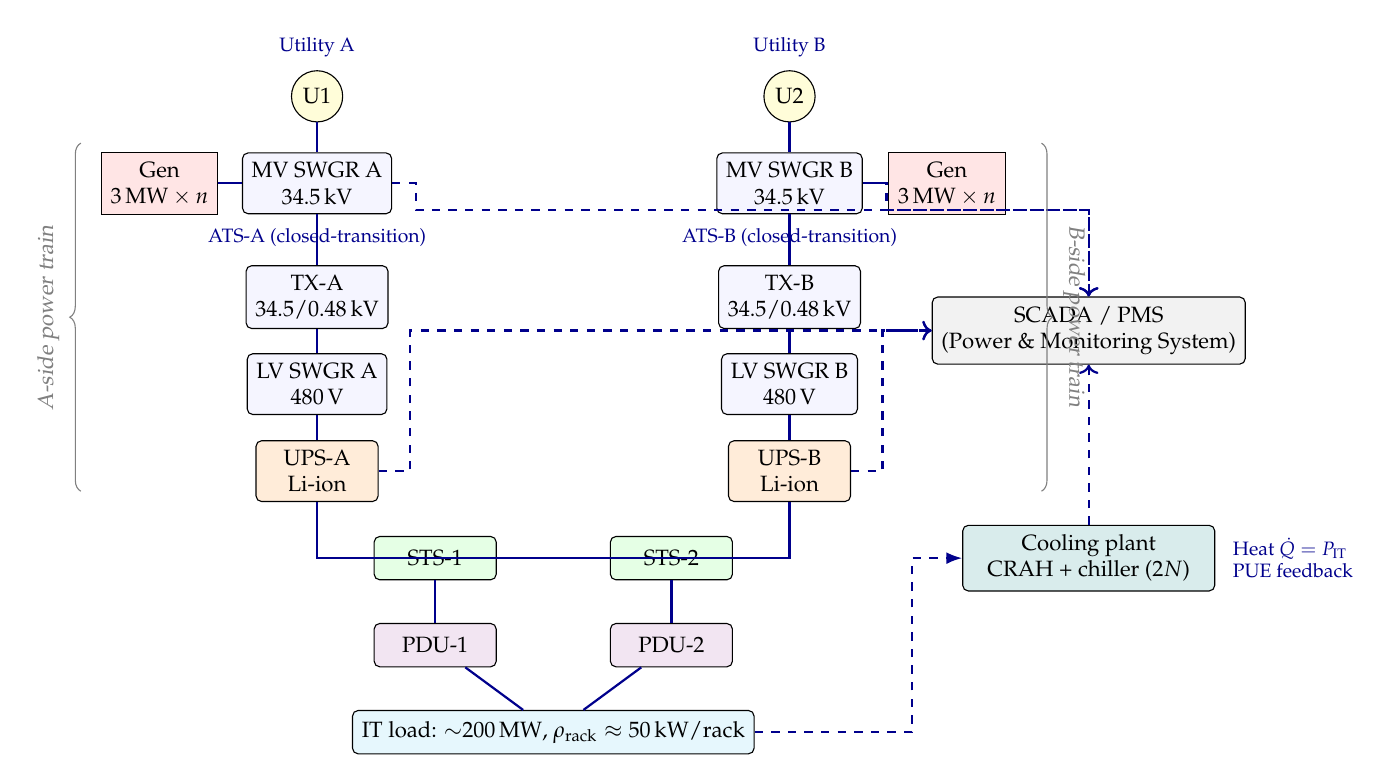
\begin{tikzpicture}[
    every node/.style={font=\footnotesize},
    blk/.style={draw,rounded corners=2pt,minimum width=1.55cm,minimum height=0.55cm,
                align=center,fill=blue!4},
    src/.style={draw,circle,minimum size=0.65cm,inner sep=0pt,fill=yellow!15},
    gen/.style={draw,rectangle,minimum width=1.05cm,minimum height=0.55cm,fill=red!10,align=center},
    bus/.style={draw,line width=1.2pt,blue!55!black},
    line/.style={-{Latex[length=2mm]},thick,blue!55!black},
    fline/.style={thick,blue!55!black},
    label/.style={font=\scriptsize,blue!55!black},
    x=1cm, y=0.85cm
]

% Utility side
\node[src] (U1) at (0,9) {U1};
\node[src] (U2) at (6,9) {U2};
\node[label,above=0.05cm of U1] {Utility A};
\node[label,above=0.05cm of U2] {Utility B};

% MV switchgear
\node[blk] (MVA) at (0,7.7) {MV SWGR A\\\SI{34.5}{\kilo\volt}};
\node[blk] (MVB) at (6,7.7) {MV SWGR B\\\SI{34.5}{\kilo\volt}};

\draw[fline] (U1) -- (MVA);
\draw[fline] (U2) -- (MVB);

% Generators / ATS
\node[gen] (G1) at (-2.0,7.7) {Gen\\ $3\,\mathrm{MW}\times n$};
\node[gen] (G2) at ( 8.0,7.7) {Gen\\ $3\,\mathrm{MW}\times n$};
\draw[fline] (G1) -- (MVA);
\draw[fline] (G2) -- (MVB);

% ATS labels
\node[label,below=0.05cm of MVA] {ATS-A (closed-transition)};
\node[label,below=0.05cm of MVB] {ATS-B (closed-transition)};

% Step-down transformers
\node[blk] (TXA) at (0,6.0) {TX-A\\$34.5/0.48$\,kV};
\node[blk] (TXB) at (6,6.0) {TX-B\\$34.5/0.48$\,kV};
\draw[fline] (MVA) -- (TXA);
\draw[fline] (MVB) -- (TXB);

% LV switchgear
\node[blk] (LVA) at (0,4.7) {LV SWGR A\\480\,V};
\node[blk] (LVB) at (6,4.7) {LV SWGR B\\480\,V};
\draw[fline] (TXA) -- (LVA);
\draw[fline] (TXB) -- (LVB);

% UPS modules
\node[blk,fill=orange!15] (UA) at (0,3.4) {UPS-A\\Li-ion};
\node[blk,fill=orange!15] (UB) at (6,3.4) {UPS-B\\Li-ion};
\draw[fline] (LVA) -- (UA);
\draw[fline] (LVB) -- (UB);

% Static transfer switches
\node[blk,fill=green!10] (STSA) at (1.5,2.1) {STS-1};
\node[blk,fill=green!10] (STSB) at (4.5,2.1) {STS-2};
\draw[fline] (UA) |- (STSA);
\draw[fline] (UB) |- (STSA);
\draw[fline] (UA) |- (STSB);
\draw[fline] (UB) |- (STSB);

% PDUs
\node[blk,fill=violet!10] (PD1) at (1.5,0.8) {PDU-1};
\node[blk,fill=violet!10] (PD2) at (4.5,0.8) {PDU-2};
\draw[fline] (STSA) -- (PD1);
\draw[fline] (STSB) -- (PD2);

% Rack loads
\node[blk,fill=cyan!10,minimum width=4.2cm] (LOAD) at (3,-0.5)
    {IT load: $\sim$\SI{200}{MW}, $\rho_{\mathrm{rack}}\approx\SI{50}{\kilo\watt\per rack}$};
\draw[fline] (PD1) -- (LOAD);
\draw[fline] (PD2) -- (LOAD);

% Cooling plant
\node[blk,fill=teal!15,minimum width=3.2cm] (COOL) at (9.8,2.1)
    {Cooling plant\\CRAH + chiller ($2N$)};
\draw[line,dashed] (LOAD.east) -- ++(2,0) |- (COOL);
\node[label,right=0.1cm of COOL,align=left]
    {Heat $\dot Q = P_{\mathrm{IT}}$\\PUE feedback};

% PMS / SCADA box
\node[blk,fill=gray!10,minimum width=3.4cm] (PMS) at (9.8,5.5)
    {SCADA / PMS\\(Power \& Monitoring System)};
\draw[line,dashed,->] (MVA.east) -- ++(0.3,0) -- ++(0,-0.4) -| (PMS);
\draw[line,dashed,->] (MVB.east) -- ++(0.3,0) -- ++(0,-0.4) -| (PMS);
\draw[line,dashed,->] (UA.east) -- ++(0.4,0) |- (PMS);
\draw[line,dashed,->] (UB.east) -- ++(0.4,0) |- (PMS);
\draw[line,dashed,->] (COOL.north) -- (PMS.south);

% Bracket: "A side" / "B side"
\draw[decorate,decoration={brace,amplitude=4pt,mirror},gray]
   (-3,8.3) -- (-3,3.1) node[midway,left=0.15cm,rotate=90,anchor=south]
   {\textsl{A-side power train}};
\draw[decorate,decoration={brace,amplitude=4pt},gray]
   (9.2,8.3) -- (9.2,3.1) node[midway,right=0.15cm,rotate=-90,anchor=south]
   {\textsl{B-side power train}};

\end{tikzpicture}
\caption{Single-line wireframe of a Tier-IV $2N$ hyperscale data center.
Solid lines are power feeders; dashed lines are SCADA telemetry. Each
half (A, B) carries 100\,\% of the design IT load, so any single
component on one side may fail or be taken out for maintenance with no
load impact. The dual independent utility feeds, dual generator
plants, dual UPS rooms and dual cooling trains are the physical
expression of the engineering $2N$ availability target of 99.995\%.}
\label{fig:singleline}
\end{figure}

\subsection{Engineering parameters that enter pricing}\label{ss:eng-params}

The underwriting-relevant electrical parameters are summarised in
Table~\ref{tab:eng-params}. They will reappear in the hazard rate
specification of \S\ref{sec:coupled}.

\begin{table}[ht]
\centering\small
\caption{Underwriting-relevant electrical engineering parameters.}\label{tab:eng-params}
\begin{tabular}{lll}
\toprule
Symbol & Quantity & Typical value (Tier IV, AI campus) \\
\midrule
$P_{\mathrm{IT}}$       & critical IT load                & \SI{50}{\mega\watt}--\SI{500}{\mega\watt} \\
$\mathrm{PUE}$          & power usage effectiveness       & $1.10$--$1.45$ (best-in-class $1.04$) \\
$\rho_{\mathrm{rack}}$  & rack power density              & \SIrange{30}{120}{\kilo\watt\per rack} \\
$T_{\mathrm{ca}}$       & cold-aisle setpoint             & \SIrange{18}{27}{\celsius} (ASHRAE A1) \\
$\eta_{\mathrm{UPS}}$   & UPS double-conversion efficiency & 0.96--0.98 \\
$\tau_{\mathrm{auto}}$  & generator autonomy on diesel    & 24--72\,h \\
$E_{\mathrm{batt}}$     & UPS battery energy              & \SIrange{5}{15}{min} of full load \\
$N_{\mathrm{cells}}$    & lithium-ion cells per UPS room  & $10^4$--$10^5$ \\
\bottomrule
\end{tabular}
\end{table}

% =========================================================================
%  cooling_section.tex
% -------------------------------------------------------------------------
%  Placeholder created on adu-00 because the file was named in the
%  GPU-spec brief but did not exist in the working tree. Replace the
%  body of this file with the cooling section text from the laptop copy
%  (fas-datart-2026) or write it directly here.
%
%  When this file is non-empty, ensure dc_paper.tex \input{}s it in the
%  right place (after the reliability section, before the SDE section).
% =========================================================================

\section{Cooling thermodynamics and the cooling-loss hazard}
\label{sec:cooling}

% TODO: prose for §4 of the working paper. Provisional skeleton:
%   - 4.1  PUE decomposition and the Carnot ceiling (eq. 4).
%   - 4.2  Wet-bulb temperature, Stull (2011) approximation (eq. 5).
%   - 4.3  Cooling-loss hazard with indicator gate (eq. 7).
%   - 4.4  Non-stationary climate process for T_{wb}(t) (eq. 12).

\subsection*{Placeholder}
The numerical results that back this section are produced by
\texttt{dcrisk.cooling} (\texttt{src/dcrisk/cooling/}) and reproduced in
\texttt{notebooks/07\_cooling\_hazard.ipynb}.


% ============================================================
\section{Reliability mathematics: from components to the site}\label{sec:reliability}

We assume the reader is familiar with the basic identity
$R(t)=\exp(-\int_0^t \lambda(s)\dd s)$ and the relationship between
failure rate $\lambda$, MTBF, MTTR and steady-state availability
\begin{equation}\label{eq:avail}
   A \;=\; \frac{\mathrm{MTBF}}{\mathrm{MTBF}+\mathrm{MTTR}},
   \qquad \mathrm{MTBF}=\frac{1}{\lambda}, \qquad U=1-A .
\end{equation}

\subsection{Fault tree representation}\label{ss:fta}

Let $T$ denote the top event ``IT load lost'' at a particular site,
and let $\{B_j\}_{j=1}^m$ denote the elementary events
(component failures, human errors, exogenous shocks). A fault tree
encodes $T$ as a Boolean function of $\{B_j\}$,
\begin{equation}\label{eq:fta-bool}
   T \;=\; \phi(B_1,\dots,B_m) .
\end{equation}
For a $2N$ topology the simplified structure is
\begin{equation}\label{eq:topdown}
   T \;\Leftrightarrow\;
   \underbrace{(E_A \wedge E_B)}_{\text{both power trains}}
   \;\vee\;
   \underbrace{(C_A \wedge C_B)}_{\text{both cooling trains}}
   \;\vee\;
   \underbrace{F_{\mathrm{cat}}}_{\text{catastrophic peril}}
   \;\vee\;
   \underbrace{Y_{\mathrm{cy}}}_{\text{cyber lockdown}},
\end{equation}
where each $E_\bullet$ is itself a series chain (utility OR generator OR
ATS OR transformer OR UPS OR PDU). Figure~\ref{fig:fta} shows the
expanded tree.

\begin{figure}[ht]
\centering
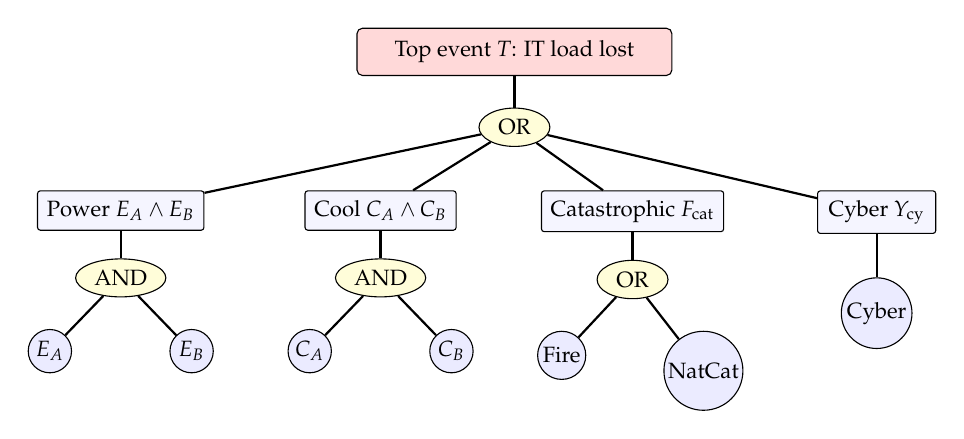
\begin{tikzpicture}[
   every node/.style={font=\footnotesize},
   top/.style={draw,rectangle,rounded corners=2pt,fill=red!15,minimum width=4cm,
               minimum height=0.6cm,align=center},
   gate/.style={draw,ellipse,fill=yellow!15,minimum width=0.9cm,minimum height=0.45cm,
                inner sep=2pt},
   bevt/.style={draw,circle,fill=blue!8,minimum size=0.55cm,inner sep=1pt,align=center},
   ievt/.style={draw,rectangle,rounded corners=1pt,fill=blue!4,minimum width=1.5cm,
                minimum height=0.5cm,align=center},
   ln/.style={thick}
]
% Top event
\node[top] (T) at (0,0) {Top event $T$: IT load lost};
\node[gate,below=0.4cm of T] (G0) {OR};
\draw[ln] (T) -- (G0);

% Four branches
\node[ievt,below=0.55cm of G0,xshift=-5.0cm] (EA) {Power $E_A\wedge E_B$};
\node[ievt,below=0.55cm of G0,xshift=-1.7cm] (CA) {Cool $C_A\wedge C_B$};
\node[ievt,below=0.55cm of G0,xshift= 1.5cm] (FC) {Catastrophic $F_{\mathrm{cat}}$};
\node[ievt,below=0.55cm of G0,xshift= 4.6cm] (CY) {Cyber $Y_{\mathrm{cy}}$};
\draw[ln] (G0) -- (EA);
\draw[ln] (G0) -- (CA);
\draw[ln] (G0) -- (FC);
\draw[ln] (G0) -- (CY);

% Power AND
\node[gate,below=0.35cm of EA] (G1) {AND};
\draw[ln] (EA) -- (G1);
\node[bevt,below=0.4cm of G1,xshift=-0.9cm] (EAfail) {$E_A$};
\node[bevt,below=0.4cm of G1,xshift= 0.9cm] (EBfail) {$E_B$};
\draw[ln] (G1) -- (EAfail);
\draw[ln] (G1) -- (EBfail);

% Cooling AND
\node[gate,below=0.35cm of CA] (G2) {AND};
\draw[ln] (CA) -- (G2);
\node[bevt,below=0.4cm of G2,xshift=-0.9cm] (CAfail) {$C_A$};
\node[bevt,below=0.4cm of G2,xshift= 0.9cm] (CBfail) {$C_B$};
\draw[ln] (G2) -- (CAfail);
\draw[ln] (G2) -- (CBfail);

% Catastrophic OR
\node[gate,below=0.35cm of FC] (G3) {OR};
\draw[ln] (FC) -- (G3);
\node[bevt,below=0.4cm of G3,xshift=-0.9cm] (FB) {Fire};
\node[bevt,below=0.4cm of G3,xshift= 0.9cm] (NC) {NatCat};
\draw[ln] (G3) -- (FB);
\draw[ln] (G3) -- (NC);

% Cyber leaf
\node[bevt,below=0.55cm of CY] (CYb) {Cyber};
\draw[ln] (CY) -- (CYb);

\end{tikzpicture}
\caption{Simplified fault tree for the top event $T=$ ``IT load lost.''
Each $E_\bullet$ is itself a series chain of elementary component
events (utility, generator, ATS, transformer, switchgear, UPS,
STS, PDU); these are not expanded here for clarity. The four top-level
branches are not independent --- a fire in the UPS room can simultaneously
fail $E_A$ and trigger fire suppression that shuts cooling.}
\label{fig:fta}
\end{figure}

\noindent For \emph{instantaneous} (steady-state) probabilities and
\emph{rare}, independent component failures,
\begin{equation}\label{eq:fta-prob}
   \Prb(T) \;\approx\; \Prb(E_A)\Prb(E_B) + \Prb(C_A)\Prb(C_B)
              + \Prb(F_{\mathrm{cat}}) + \Prb(Y_{\mathrm{cy}}),
\end{equation}
where each $\Prb(E_\bullet)=1-\prod_k (1-q_k)$ for the relevant series
chain of unavailabilities $q_k$. The independence assumption is
abandoned in \S\ref{sec:dependence}.

\subsection{Markov chain of plant states}\label{ss:markov}

A more dynamic representation is the continuous-time Markov chain
$\{Z_t\}$ on
\begin{equation}
   \mathcal{S} = \{\,
       \mathrm{OK},\;\mathrm{Deg}_1,\;\mathrm{Deg}_2,\;\mathrm{F}\,\},
\end{equation}
corresponding to (both trains healthy, one train down,
both trains down on one subsystem, total failure). For a $2N$ site:

\begin{figure}[ht]
\centering
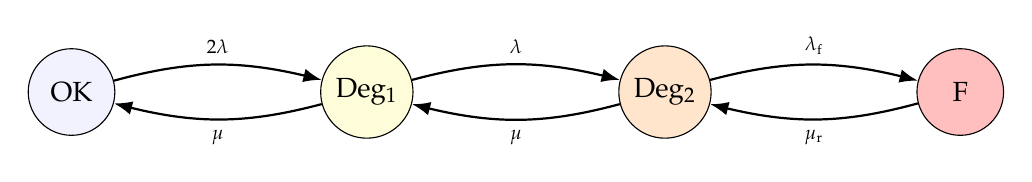
\begin{tikzpicture}[
  node distance=2.2cm and 2.6cm,
  state/.style={draw,circle,minimum size=1.1cm,fill=blue!5},
  every edge/.style={draw,thick,->,>=Latex}
]
\node[state] (S0) {OK};
\node[state,right=of S0,fill=yellow!15] (S1) {Deg$_1$};
\node[state,right=of S1,fill=orange!20] (S2) {Deg$_2$};
\node[state,right=of S2,fill=red!25] (SF) {F};

\draw (S0) edge[bend left=15] node[above,font=\scriptsize] {$2\lambda$} (S1);
\draw (S1) edge[bend left=15] node[below,font=\scriptsize] {$\mu$} (S0);
\draw (S1) edge[bend left=15] node[above,font=\scriptsize] {$\lambda$} (S2);
\draw (S2) edge[bend left=15] node[below,font=\scriptsize] {$\mu$} (S1);
\draw (S2) edge[bend left=15] node[above,font=\scriptsize] {$\lambda_{\mathrm{f}}$} (SF);
\draw (SF) edge[bend left=15] node[below,font=\scriptsize] {$\mu_{\mathrm{r}}$} (S2);
\end{tikzpicture}
\caption{Continuous-time Markov chain on plant states for a $2N$
data center. $\lambda$: per-train degradation rate. $\mu$: per-train
repair rate. $\lambda_{\mathrm{f}}$: degraded-to-failed rate, which is
dramatically higher than $\lambda$ because the system has lost
fault tolerance. $\mu_{\mathrm{r}}$: full-site restoration rate.}
\label{fig:markov}
\end{figure}

\noindent The steady-state distribution $\bm{\pi}=(\pi_0,\pi_1,\pi_2,\pi_F)$
solves $\bm\pi\, \mathbf{Q}=\mathbf{0}$, $\bm\pi\mathbf{1}=1$,
where the generator is
\begin{equation}\label{eq:Qmatrix}
\mathbf{Q} =
\begin{pmatrix}
-2\lambda & 2\lambda  & 0                       & 0 \\
\mu       & -(\mu+\lambda) & \lambda            & 0 \\
0         & \mu       & -(\mu+\lambda_{\mathrm f}) & \lambda_{\mathrm f}\\
0         & 0         & \mu_{\mathrm r}         & -\mu_{\mathrm r}
\end{pmatrix} .
\end{equation}
The unavailability $U=\pi_F$ admits a closed-form expression that we
can equate to $1-A$ from Table~\ref{tab:tier}; this calibration
identifies the per-component $\lambda$ once $\mu$ and $\mu_{\mathrm r}$
are fixed by site operating procedures.

\begin{proposition}\label{prop:avail}
For the chain in Figure~\ref{fig:markov} with $\lambda\ll\mu$, the
steady-state unavailability satisfies, to leading order,
\begin{equation}\label{eq:U-leading}
   U \;\approx\; \frac{2\lambda^2 \lambda_{\mathrm f}}{\mu^2 \mu_{\mathrm r}}.
\end{equation}
\end{proposition}

\begin{proof}[Sketch]
With $\lambda\ll\mu$, the chain is heavily attracted to OK. Standard
results from \citet{Trivedi2017} give
$\pi_1\approx 2\lambda/\mu$, $\pi_2\approx 2\lambda^2/\mu^2$,
$\pi_F\approx 2\lambda^2 \lambda_{\mathrm f}/(\mu^2\mu_{\mathrm r})$.
\end{proof}

\noindent Equation~\eqref{eq:U-leading} is the bridge from electrical
engineering specifications to actuarial frequency: ageing of any
component drives $\lambda$ up multiplicatively, and the cube of those
rates appears in $U$. The framework is exquisitely sensitive to
component reliability --- exactly the underwriting result needed.

\subsection{From availability to claim frequency}\label{ss:freq-from-A}

If we declare a ``site outage event'' to be any visit by $\{Z_t\}$ to
$\mathrm{F}$, the number of such visits in $[0,1]$ year is, in steady
state, well-approximated by a Poisson process with intensity
\begin{equation}\label{eq:freq-from-A}
   \lambda^{\mathrm{out}} \;=\; \pi_2 \, \lambda_{\mathrm f}
   \;\approx\; \frac{2\lambda^2 \lambda_{\mathrm f}}{\mu^2}\;
   \text{per year}.
\end{equation}
This is our \emph{engineering-derived prior} on actuarial frequency. We
will see in \S\ref{sec:freq} how to update it from empirical claims
data.


% ============================================================
\section{The coupled power--thermal--cyber failure model}\label{sec:coupled}

\subsection{State space and dynamics}

The novelty of our framework is to treat the data center as a
\emph{coupled multi-physics system} rather than as a collection of
independent components. Let
\begin{equation}\label{eq:state}
   \mathbf{X}_t \;=\;
   \bigl(V_t,\; T_t,\; C_t\bigr)^{\top}\in \R^3,
\end{equation}
where
\begin{itemize}[leftmargin=*,nosep]
  \item $V_t$: the prevailing per-unit bus voltage at the main LV
        switchgear ($V_t\equiv 1$ in normal operation),
  \item $T_t$: the cold-aisle return temperature deviation above setpoint
        (\si{\kelvin}),
  \item $C_t$: an abstract cyber-load process (e.g.\ rate of
        intrusion attempts per second, log-transformed).
\end{itemize}

\noindent We posit the following stochastic differential equations:

\begin{equation}\label{eq:sde}
\boxed{
\begin{aligned}
   \dd V_t &= -\kappa_V\bigl(V_t-1\bigr)\,\dd t
            + \sigma_V\,\dd W^{V}_t
            - J^V_t\,\dd N^{V}_t , \\[2pt]
   \dd T_t &= \alpha\,\bigl[g(V_t)\,P_{\mathrm{IT}}
                            - q(\mathrm{PUE})\,c(V_t)\bigr]\dd t
            + \sigma_T\,\dd W^{T}_t , \\[2pt]
   \dd C_t &= \kappa_C\bigl(\bar c - C_t\bigr)\dd t + \sigma_C\,\dd W^{C}_t,
\end{aligned}}
\end{equation}
with independent standard Brownian motions
$(W^V,W^T,W^C)$ subject to the correlation
$\dd W^{V}\dd W^{T}=\rho_{VT}\dd t$,
$\dd W^{T}\dd W^{C}=\rho_{TC}\dd t$,
$\dd W^{V}\dd W^{C}=\rho_{VC}\dd t$, all initialised at
$\mathbf{X}_0=(1,0,\bar c)$, and where
$N^V_t$ is a Poisson process counting upstream voltage-sag events with
intensity $\beta_V$.

\paragraph{Reading the model.}
\begin{itemize}[leftmargin=*,nosep]
  \item The voltage equation is an Ornstein--Uhlenbeck process pulled
        back to nominal ($V=1$), perturbed by Gaussian small-signal noise
        $\sigma_V \dd W^V$ and discrete sag-jumps $J^V_t$ of random size at
        rate $\beta_V$. Real SCADA voltage traces are well-modelled in
        this form.
  \item In the thermal equation, the function
        $g(v)=1\!\!\1_{\{v>v_{\min}\}}$ acts as a binary indicator that
        IT continues to draw rated power above the UPS dropout
        threshold $v_{\min}$, while $c(v)$ is the cooling-system
        capacity which collapses below the same threshold (cooling
        plant pulled off-grid).
        The parameter $q(\mathrm{PUE})=(\mathrm{PUE}-1)\,P_{\mathrm{IT}}$
        converts the facility overhead into reject heat. $\alpha$ is
        the lumped thermal capacitance of the white space.
  \item The cyber-load equation is again Ornstein--Uhlenbeck, capturing
        the noisy background of intrusion attempts. Spikes are
        modelled via a separately-counted compound Poisson process below.
\end{itemize}

\subsection{Coupled instantaneous failure hazard}

The instantaneous hazard rate that the IT critical load is lost in
the next time-step combines three accelerative effects:
\begin{equation}\label{eq:hazard}
   \boxed{\;
   \lambda_t \;=\; \underbrace{\lambda_0\, e^{-E_a/k_B T_t}}_{\text{Arrhenius thermal}}
   \cdot \underbrace{\bigl(\tfrac{V_t}{V_{\mathrm{nom}}}\bigr)^{-\gamma_V}}_{\text{voltage-stress}}
   \cdot \underbrace{\exp(\beta_C\,C_t)}_{\text{cyber-stress}} .\;}
\end{equation}
The Arrhenius factor comes from the standard semiconductor reliability
acceleration model: $E_a$ is an effective activation energy (typically
$0.6\,$--$\,0.9$\,eV for IC failures), $k_B$ is Boltzmann's constant.
A $\Delta T=\SI{10}{\kelvin}$ rise above setpoint roughly halves
component MTBF~\citep{Black1969}, which is the headline industrial
``10\,°C rule.''

The voltage-stress factor reflects accelerated insulation ageing
with $\gamma_V\in[3,7]$ for liquid-filled transformers under the
Arrhenius--inverse-power-law (AIPL) model.

The cyber-stress factor is the cleanest novelty: an Esscher-style
exponential tilt of the baseline rate by the prevailing cyber-load.

\subsection{Catastrophic transitions as first-hitting times}

A subset of catastrophic events are best modelled not as smooth
hazard increases but as the first time a state variable crosses a
critical boundary.

\begin{definition}[Thermal runaway hitting time]\label{def:hit}
Define the thermal runaway barrier
$T^* = T_{\mathrm{runaway}}-T_{\mathrm{setpoint}}$, e.g.\
$T^*\approx \SI{40}{\kelvin}$ for Li-ion NMC chemistry. The thermal
runaway hitting time is
\begin{equation}\label{eq:hitting}
   \tau^* \;=\; \inf\{\,t>0 : T_t \geq T^*\,\}.
\end{equation}
\end{definition}

For the thermal SDE in~\eqref{eq:sde} the distribution of $\tau^*$
solves the Kolmogorov backward equation; under mean-reverting drift it
is well-approximated by an inverse-Gaussian distribution
\citep{Chhikara1989}:
\begin{equation}\label{eq:IG}
   \tau^* \sim \mathrm{IG}(\mu_{\tau},\,\lambda_{\tau}),\qquad
   f_{\tau^*}(t) \;=\;
   \sqrt{\tfrac{\lambda_{\tau}}{2\pi t^{3}}}\,
   \exp\!\left\{-\tfrac{\lambda_{\tau}(t-\mu_{\tau})^2}{2\mu_{\tau}^2 t}\right\},
\end{equation}
with mean $\mu_\tau=T^*/\alpha\,\E[\text{net heat in}]$ and shape
$\lambda_\tau$ identified from $\sigma_T$ and the boundary distance.

\subsection{Deterministic limit: the operator's grace period}
\label{ss:tcrit}

The stochastic first-hitting characterisation has a clean
deterministic counterpart that engineers reach for first and that
operators actually use in pre-incident drills. Setting $\sigma_T\!\to\! 0$
and $V_t\equiv 1$ in~\eqref{eq:sde} reduces the thermal equation
to the lumped-capacitance heat balance
\begin{equation}\label{eq:lumped}
   m\,c_p\,\frac{\dd T(t)}{\dd t}
   \;=\; Q_{\mathrm{IT}} \;-\; UA\,\bigl(T(t)-T_{\mathrm{amb}}\bigr),
\end{equation}
where $m$ (kg) and $c_p$ (J\,kg$^{-1}$K$^{-1}$) are the lumped mass
and specific heat of air and structure in the white space, $UA$
(W\,K$^{-1}$) is the lumped envelope conductance, $Q_{\mathrm{IT}}=P_{\mathrm{IT}}$
is the IT reject heat and $T_{\mathrm{amb}}$ is the ambient outdoor
temperature. Equation~\eqref{eq:lumped} is a linear first-order ODE
with closed-form solution
\begin{equation}\label{eq:Tt}
   T(t) \;=\; \underbrace{T_{\mathrm{amb}}+\tfrac{Q_{\mathrm{IT}}}{UA}}_{T_\infty}
   \;+\;\Bigl(T_0-T_{\mathrm{amb}}-\tfrac{Q_{\mathrm{IT}}}{UA}\Bigr)\,
   \exp\!\Bigl(-\tfrac{UA}{m c_p}\,t\Bigr).
\end{equation}
Note that for a typical hyperscale hall in cooling-failure mode,
$Q_{\mathrm{IT}}/UA$ is far above any safe room temperature: cooling
\emph{must} resume before the asymptote $T_\infty$ is approached.
Solving~\eqref{eq:Tt} for the first time $T$ reaches the ASHRAE A1
operating limit $T_{\mathrm{crit}}$ (\SI{32}{\celsius} for general use)
gives the \textbf{deterministic grace period}
\begin{equation}\label{eq:tcrit}
   \boxed{\;
   t_{\mathrm{crit}} \;=\; -\,\frac{m c_p}{UA}\,
   \ln\!\left(
     \frac{T_{\mathrm{crit}}-T_{\mathrm{amb}}-Q_{\mathrm{IT}}/UA}
          {T_0-T_{\mathrm{amb}}-Q_{\mathrm{IT}}/UA}
   \right).\;}
\end{equation}
The stochastic counterpart $\tau^*$ from \eqref{eq:hitting}--\eqref{eq:IG}
is well-approximated by a distribution centred at $t_{\mathrm{crit}}$
with dispersion driven by $\sigma_T$.

\begin{rbox}
For a typical \SI{20}{\mega\watt} IT hall ($Q_{\mathrm{IT}}=\SI{20}{MW}$),
$m c_p \approx 3.5\times 10^{6}$\,J/K, $UA\approx 10^{4}$\,W/K,
$T_0=\SI{22}{\celsius}$, $T_{\mathrm{amb}}=\SI{30}{\celsius}$,
$T_{\mathrm{crit}}=\SI{32}{\celsius}$, \eqref{eq:tcrit} gives
$t_{\mathrm{crit}}\approx 3.5\,\mathrm{minutes}$. This is the
engineering reality that drives the $24/7$ rotation of redundant
chillers, and the actuarial reality that even Tier-IV sites with
\SI{15}{minute} battery autonomy are running closer to the cooling
boundary than to the power boundary.
\end{rbox}

\begin{nbox}
\textbf{Why this matters.} Treating thermal runaway as a first-hitting
time means the protective effect of \emph{off-gas detection} (which
shifts the boundary $T^*$ effectively to a lower temperature $T^*_\mathrm{eff}$
because mitigation can be applied earlier) enters the model
\emph{multiplicatively in the hazard}, not additively in the loss.
This explains why off-gas detection retrofits have been observed to
move site-level loss costs by 40--60\,\%, far more than a naive
reduction-in-frequency calculation predicts: the lengthened tail of
$\tau^*$ removes precisely the most extreme right tail of the loss
distribution.
\end{nbox}

% ============================================================
\section{Frequency modelling}\label{sec:freq}

\subsection{Annual count of insurable outages}

Let $N_i$ be the number of outage events at site $i$ in a policy
year. The naïve actuarial benchmark is the homogeneous Poisson
\begin{equation}\label{eq:Poi}
   N_i \,\sim\, \mathrm{Poisson}(\lambda_i),\qquad
   \E[N_i]=\Var(N_i)=\lambda_i .
\end{equation}
Empirical experience with multi-site portfolios overwhelmingly
shows over-dispersion ($\Var/\E\!>\!1$), driven by site
heterogeneity in operational maturity, climate exposure and
equipment age. We therefore adopt a \textbf{Poisson--Gamma frailty}
mixed model:
\begin{equation}\label{eq:NB}
   N_i \given \Theta_i \,\sim\, \mathrm{Poisson}(\lambda_i \Theta_i),
   \qquad \Theta_i \stackrel{\mathrm{iid}}{\sim} \mathrm{Gamma}(\nu,\nu),
\end{equation}
which marginally yields a Negative Binomial
$N_i\sim\mathrm{NB}\bigl(\nu,\,\nu/(\nu+\lambda_i)\bigr)$ with
\begin{equation}
   \E[N_i]=\lambda_i,\qquad
   \Var(N_i)=\lambda_i\bigl(1+\lambda_i/\nu\bigr).
\end{equation}

\subsection{The frequency regression}\label{ss:freq-reg}

The site-specific rate $\lambda_i$ is parameterised log-linearly in
underwriting covariates:
\begin{equation}\label{eq:GLM}
   \log \lambda_i \;=\; \beta_0
   + \beta_1 \log P_{\mathrm{IT},i}
   + \beta_2 \,\bigl(\mathrm{PUE}_i - 1\bigr)
   + \beta_3 \,\mathrm{Age}_i
   + \beta_4 \,\1\{\mathrm{Tier}<\mathrm{IV}\}_i
   + \beta_5 \,\mathrm{ClimateScore}_i .
\end{equation}
The coefficient on PUE deserves attention: \emph{higher PUE means more
of the energy budget is lost to mechanical and electrical overhead}.
Empirically this co-varies with cooling stress and with lower-quality
equipment. We expect $\beta_2 > 0$. The IT-load coefficient absorbs
the simple intuition that bigger sites have more components and
therefore more failure opportunities, but \emph{economies of redundancy}
typically push $\beta_1 < 1$.

\subsection{Engineering prior, statistical posterior}

Equation~\eqref{eq:freq-from-A} gives the engineering prior
$\lambda_i^{\mathrm{out},\mathrm{eng}}$ from the Tier-class
availability. In a Bayesian setting, we treat it as the prior mean and
update with claims experience $\mathbf{D}_i=\{n_{i,t},t=1,\dots,T\}$:
\begin{equation}\label{eq:bayes}
   \pi(\lambda_i \given \mathbf{D}_i)
   \;\propto\; \pi(\lambda_i)\,\prod_{t=1}^{T}
   \frac{(\lambda_i)^{n_{i,t}} e^{-\lambda_i}}{n_{i,t}!} .
\end{equation}
If the prior is Gamma, this is conjugate and gives a closed-form
posterior. This is precisely the \emph{credibility} framework of
B\"uhlmann--Straub, with the engineering prior playing the role of
the collateral information.

\begin{rbox}
\textbf{Cox/doubly-stochastic structure.} The Poisson--Gamma frailty
in~\eqref{eq:NB} is precisely a \emph{doubly stochastic} (Cox) Poisson
process: the intensity $\lambda_i\Theta_i$ is itself random, drawn at
the site level. If we let the intensity depend on time-varying
covariates such as $T_{\mathrm{amb}}(t)$, the model generalises naturally to
\begin{equation*}
   \lambda_i(t) \;=\; \lambda_i \cdot
   \exp\!\bigl(\gamma_1 \max(0,T_{\mathrm{amb}}(t)-T_{\mathrm{design}})
              + \gamma_2 \1_{\{Z_t=\mathrm{Deg}_2\}}\bigr),
\end{equation*}
which couples the actuarial frequency directly to the Markov chain
state of \S\ref{ss:markov} and to a meteorological covariate. The
unconditional claim count is then a Cox process whose intensity
inherits the dynamics of both the plant and the weather.
\end{rbox}

% ============================================================
\section{Severity modelling and the tail}\label{sec:severity}

\subsection{Compound aggregate loss}

Total annual loss for site $i$ is the compound random variable
\begin{equation}\label{eq:S}
   S_i \;=\; \sum_{j=1}^{N_i} X_{i,j},\qquad
   X_{i,j}\stackrel{\mathrm{iid}}{\sim}F_X.
\end{equation}
Both the mean and variance of $S_i$ are given by
Wald's identities:
\begin{align}
   \E[S_i] &= \E[N_i]\,\E[X],\\
   \Var(S_i) &= \E[N_i]\,\Var(X) + \Var(N_i)\,\E[X]^2.
\end{align}
For the NB frequency assumption, the second identity becomes
\begin{equation}\label{eq:varS-NB}
   \Var(S_i) \;=\; \lambda_i\,\E[X^2] +
                  \frac{\lambda_i^2}{\nu}\,\E[X]^2 ,
\end{equation}
making explicit how frailty inflates the variance over the Poisson case.

\subsection{Body--tail severity decomposition}

The severity distribution $F_X$ has a markedly bimodal character:
\begin{itemize}[leftmargin=*,nosep]
  \item \textbf{Attritional losses} (PDU failures, single rack burns,
        short cooling excursions) cluster around \$100k--\$5M and
        fit a lognormal body very well.
  \item \textbf{Catastrophic losses} (full-site fire, total power
        train loss, lithium-ion cascading event) are heavy-tailed and
        follow a power law.
\end{itemize}
We adopt a \emph{Peaks-over-Threshold} (POT) decomposition: choose a
threshold $u$ (e.g.\ the 95th percentile of historical claims), and model
\begin{equation}\label{eq:POT}
   F_X(x) \;=\;
   \begin{cases}
      F_{\mathrm{body}}(x), & x < u, \\[3pt]
      1 - (1-F_X(u))\Bigl[1 + \xi\dfrac{x-u}{\sigma}\Bigr]^{-1/\xi}, & x \geq u .
   \end{cases}
\end{equation}
The tail is a Generalised Pareto with shape $\xi$ and scale
$\sigma$, justified by the Pickands--Balkema--de~Haan theorem
\citep{Balkema1974,Pickands1975}: for any distribution in the maximum
domain of attraction of an extreme value distribution, exceedances
above a high enough threshold converge to a GPD. Maximum-likelihood
estimates of $\xi$ for data-center catastrophic losses are typically
in the $\xi\in(0.2,0.6)$ range --- meaningfully heavy-tailed.

\subsection{Probable Maximum Loss and Maximum Foreseeable Loss}

Lenders and reinsurers reference two engineering loss metrics adapted
to data centers:
\begin{align}
   \mathrm{PML}_\alpha &\;=\; \VaR_\alpha(X\given X>u)
   \;=\; u + \frac{\sigma}{\xi}
        \Bigl[\bigl(\tfrac{1-\alpha}{p_u}\bigr)^{-\xi}-1\Bigr], \label{eq:PML}\\
   \mathrm{MFL}      &\;=\; \text{deterministic worst credible loss assuming all controls fail.}
\end{align}
For a $\xi=0.4$, $\sigma=\$50M$, $u=\$10M$ tail and $\alpha=99.5\%$
with $p_u=0.05$, the PML works out to about \$870M --- consistent with
broker estimates for a \SI{100}{\mega\watt} Tier-III site.

\subsection{Operationalising BI severity via SLA structure}
\label{ss:BI-SLA}

The pure-statistical severity above tells us \emph{how big} a loss is
but says nothing about \emph{why}. For data center operators, the
loss decomposition~\eqref{eq:loss-decomp} contains an item
$L^{(i)}_{\mathrm{BI}}$ whose magnitude is governed by an SLA contract
between the operator and its tenants. A single outage of length
$\tau$ generates a piecewise BI loss
\begin{equation}\label{eq:BI-piece}
   \boxed{\;
   X^{\mathrm{BI}}(\tau) \;=\;
   C_{\mathrm{SLA}}\,\max\!\bigl(0,\,\tau-\tau_0\bigr)
   \;+\; \kappa\,\1\{\tau > t_{\mathrm{crit}}\}
   \;+\; \rho_{\mathrm{churn}}\,\tau^2 \,,\;}
\end{equation}
with the interpretation
\begin{itemize}[leftmargin=*,nosep]
  \item $\tau_0$: the SLA-permitted deductible window
        (e.g.\ ``five nines'' $\Rightarrow \tau_0\approx 5.26$\,min/yr).
  \item $C_{\mathrm{SLA}}$: contractual penalty rate per unit downtime
        above $\tau_0$ (US\$/min). Most colocation contracts set
        $C_{\mathrm{SLA}}$ to one to three monthly recurring revenue (MRR)
        equivalents per cumulative downtime quarter, with caps.
  \item $\kappa$: a step penalty triggered the moment downtime exceeds
        the thermodynamic grace period $t_{\mathrm{crit}}$ derived in
        \eqref{eq:tcrit}; this is where ``customers start migrating''
        in real-world incident accounts.
  \item $\rho_{\mathrm{churn}}\,\tau^2$: a quadratic churn term
        capturing the empirical fact that the marginal customer-loss
        rate grows with downtime, not stays flat.
\end{itemize}

\noindent The BI duration $\tau$ itself is well-modelled as
lognormal, $\ln\tau\sim\mathcal{N}(\mu_\tau,\sigma_\tau^2)$, calibrated
from MTTR experience. Combining with~\eqref{eq:BI-piece} and integrating
out $\tau$ gives a closed-form $\E[X^{\mathrm{BI}}]$ in terms of the
lognormal CDF $\Phi$, useful for fast quotation:
\begin{equation}\label{eq:BI-mean}
\begin{aligned}
   \E[X^{\mathrm{BI}}] \;=\;{}&
   C_{\mathrm{SLA}}\bigl[\,e^{\mu_\tau+\sigma_\tau^2/2}\bar\Phi(z_0)
     - \tau_0\,\bar\Phi(z_0')\,\bigr] \\[2pt]
   &+\;\kappa\,\bar\Phi(z_{\mathrm{crit}}')
   \;+\;\rho_{\mathrm{churn}}\,e^{2\mu_\tau+2\sigma_\tau^2},
\end{aligned}
\end{equation}
with $z_0=(\ln\tau_0-\mu_\tau-\sigma_\tau^2)/\sigma_\tau$, primed
versions at $\sigma_\tau^2=0$, and $\bar\Phi=1-\Phi$. The actuarial
contribution of the $\kappa$ term is highly non-linear in
$t_{\mathrm{crit}}$, which links underwriting directly to the
engineering parameters $m c_p$ and $UA$ from~\eqref{eq:tcrit}.

% ============================================================
\section{Cyber--physical dependence via copula}\label{sec:dependence}

\subsection{Why independence fails}

Cyber incidents and physical failures are not independent. Three
empirical mechanisms link them: (i) a successful intrusion of the
Building Management System can deliberately mis-set cooling
controls; (ii) physical events (a fire, a flood) often disable
cyber-defence appliances along with everything else; (iii) major
cyber-events and major physical events both correlate with
operational human-factor stress (peak utilisation, contractor
activity).

\subsection{Gaussian copula linkage}

Let $S^{\mathrm{phy}}_i$ and $S^{\mathrm{cy}}_i$ be the marginal annual
loss aggregates from physical and cyber peril streams, with marginal
CDFs $F^{\mathrm{phy}}$ and $F^{\mathrm{cy}}$. We link them via a
bivariate Gaussian copula:
\begin{equation}\label{eq:copula}
   C_\rho(u_1,u_2) \;=\; \Phi_2\bigl(\Phi^{-1}(u_1),\Phi^{-1}(u_2);\rho\bigr),
\end{equation}
so that the joint distribution is
\begin{equation}
   F(s_1,s_2) \;=\; C_\rho\bigl(F^{\mathrm{phy}}(s_1),\,F^{\mathrm{cy}}(s_2)\bigr).
\end{equation}
The total site loss is then $S_i = S^{\mathrm{phy}}_i + S^{\mathrm{cy}}_i$,
with variance
\begin{equation}\label{eq:totalvar}
   \Var(S_i) \;=\; \Var(S^{\mathrm{phy}}_i) + \Var(S^{\mathrm{cy}}_i)
                 + 2\rho\sqrt{\Var(S^{\mathrm{phy}}_i)\Var(S^{\mathrm{cy}}_i)} .
\end{equation}

\begin{rbox}
The Gaussian copula is a starting point but is asymptotically tail
\emph{independent}, which means it understates joint extremes. For the
tail layer of a reinsurance treaty, a t-copula with low degrees of
freedom (e.g.\ $\nu=4$) or a Gumbel copula is preferable. The
calibration data are scarce; expert elicitation of
$\tau_{\mathrm{Kendall}}=0.15$--$0.25$ is a reasonable industry prior.
\end{rbox}

\subsection{Gumbel copula for the tail layer}\label{ss:gumbel}

The Gaussian-copula tail-independence defect is repaired with an
Archimedean Gumbel copula
\begin{equation}\label{eq:gumbel}
   C_\theta(u_1,u_2) \;=\;
   \exp\!\left\{-\bigl[(-\ln u_1)^{\theta} + (-\ln u_2)^{\theta}\bigr]^{1/\theta}\right\},
   \qquad \theta \ge 1,
\end{equation}
where $\theta=1$ recovers independence and $\theta\to\infty$ yields
perfect comonotonicity. The Gumbel admits asymptotic upper tail
dependence
\begin{equation}\label{eq:lambdaU}
   \lambda_U \;=\; \lim_{u\uparrow 1}
   \Prb\bigl(U_2>u\given U_1>u\bigr)
   \;=\; 2 - 2^{1/\theta}\,,
\end{equation}
so that $\theta=1.5$ yields $\lambda_U\approx 0.41$ and $\theta=3$
yields $\lambda_U\approx 0.74$. Kendall's $\tau$ is related to
$\theta$ by the closed form $\tau_K = 1 - 1/\theta$, which is how the
expert prior $\tau_K\in(0.15,0.25)$ translates into
$\theta\in(1.18,1.33)$, hence $\lambda_U\in(0.20,0.31)$ ---
a substantial joint-tail probability that the Gaussian copula assigns
the value zero. The Gumbel is therefore our recommended choice for
layers attaching at the 1-in-50 level and above, with the Gaussian
retained for the attritional layer where the bulk of the data lives.

% ============================================================
\section{Pricing}\label{sec:pricing}

\subsection{Surplus process and the Cram\'er--Lundberg framing}
\label{ss:surplus}

Before computing premiums it is useful to fix the underlying surplus
dynamics. For a portfolio absorbing the aggregate loss
$S(t)=\sum_{j=1}^{N(t)}X_j$ at rate set by the Cox intensity of
\S\ref{sec:freq}, the insurer's surplus evolves as
\begin{equation}\label{eq:CL}
   U(t) \;=\; u_0 \;+\; \Pi\,t \;-\; S(t),
\end{equation}
where $u_0$ is initial capital and $\Pi$ is the constant premium rate.
The probability of ultimate ruin
$\psi(u_0)=\Prb\bigl(\inf_{t\ge 0}U(t)<0\bigr)$ is bounded above by
Lundberg's inequality $\psi(u_0)\le e^{-Ru_0}$ for the adjustment
coefficient $R$ solving $\E[e^{R X}]=1+\Pi R/\lambda$. In the
data-center context, $R$ is small (heavy-tailed $X$) and Lundberg's
bound is loose, which is precisely why we move to the variance- and
tail-based loading principles below rather than rely on classical ruin
theory.

\subsection{The pure premium}

The pure (or risk) premium per site per year is
\begin{equation}\label{eq:pure}
   P^{\mathrm{pure}}_i \;=\; \E[S_i]
   \;=\; \E[N_i]\cdot\E[X]
   \;=\; \lambda_i\,\E[X] .
\end{equation}
For sites in a portfolio $\mathcal{I}$, the portfolio pure premium is
$\sum_i P^{\mathrm{pure}}_i$.

\subsection{Risk loading principles}\label{ss:loadings}

A pure premium does not compensate the insurer for taking on the
volatility around $\E[S_i]$. The technical premium adds a
\emph{risk load} $\Pi_{\mathrm{load}}$. We present four widely used
principles and their interpretation:

\paragraph{Standard deviation principle.}
\begin{equation}\label{eq:sdp}
   P^{\mathrm{SD}}_i \;=\; \E[S_i] + \theta\,\mathrm{SD}(S_i),
   \qquad \theta>0.
\end{equation}
Simple, but does not distinguish upside from downside.

\paragraph{Variance principle.}
\begin{equation}\label{eq:vp}
   P^{\mathrm{V}}_i \;=\; \E[S_i] + a\,\Var(S_i),\qquad a>0,
\end{equation}
which penalises portfolios with heavy tails more aggressively.

\paragraph{Esscher transform.}
For a parameter $h>0$,
\begin{equation}\label{eq:esscher}
   P^{\mathrm{E}}_i \;=\;
   \frac{\E[\,S_i\,e^{h S_i}]}{\E[\,e^{h S_i}]}.
\end{equation}
The Esscher principle has the appealing property of being additive on
independent risks and corresponds to a change-of-measure construction
naturally arising in financial mathematics.

\paragraph{Wang transform.}
The Wang transform~\citep{Wang2000} adjusts the survival function
$\bar F_S(s)=1-F_S(s)$ via
\begin{equation}\label{eq:wang}
   \bar F^{*}_S(s) \;=\; \Phi\bigl(\Phi^{-1}\!\bigl(\bar F_S(s)\bigr) + \lambda^*\bigr),
\end{equation}
and prices by $P^{\mathrm{W}}_i=\int_0^\infty \bar F^{*}_{S_i}(s)\dd s$.
The Wang transform produces the same prices as CAPM in the normal
case and the same prices as Black--Scholes for log-normal payoffs ---
making it the natural choice for hybrid insurance/capital-markets
structures (cat bonds, ILS) that are likely to absorb data center
peak-layer risk over time.

\subsection{Loading the data-center book}

We propose a hybrid loading:
\begin{equation}\label{eq:final}
   \boxed{\;
   P^{\mathrm{tech}}_i \;=\; \E[S_i]
   \;+\; \theta_1 \mathrm{SD}(S^{\mathrm{attr}}_i)
   \;+\; \theta_2 \bigl[\TVaR_{0.995}(S^{\mathrm{cat}}_i)-\E[S^{\mathrm{cat}}_i]\bigr] ,\;}
\end{equation}
splitting the attritional layer (low $\theta_1\approx 0.3$ standard
deviation load) from the catastrophic layer (high $\theta_2\approx 0.15$
Tail-VaR-based load). This mirrors the actual reinsurance market's
treatment.

% ============================================================
\section{Hybrid indemnity--parametric product}\label{sec:product}

\subsection{Trigger architecture}

Pure indemnity products on data centers are slow to settle (complex
forensics on equipment), inflate basis between sites, and bake in
ex-post adversarial information asymmetry. Pure parametric products
remove these frictions but introduce basis risk. We propose a
\textbf{three-layer hybrid}:

\smallskip
\begin{tcolorbox}[colback=blue!4,colframe=blue!55!black,title=Hybrid product]
\begin{description}
  \item[Layer 1 (parametric, fast).] Triggered automatically by SCADA
        measurements of $T_t$, $V_t$ exceeding pre-agreed thresholds
        for pre-agreed durations. Settled in days.
  \item[Layer 2 (parametric, cyber-trigger).] Triggered by detection
        of cloud outage or measured downtime of named SaaS/PaaS/IaaS
        services exceeding a threshold, as already implemented by
        Parametrix~\citep{Parametrix2022}.
  \item[Layer 3 (indemnity).] Catastrophic property/BI/SLA layer for
        residual basis. Slower, larger limits, and reinsured via
        excess-of-loss treaties.
\end{description}
\end{tcolorbox}

\subsection{Basis risk decomposition}

For Layer~1, basis risk is measured by
\begin{equation}\label{eq:basis}
   \mathrm{BR}_i \;=\;
   \E\!\left[\,\bigl(L^{\mathrm{actual}}_i - L^{\mathrm{param}}_i\bigr)^2\right],
\end{equation}
which can be decomposed as
\begin{equation}\label{eq:basis2}
   \mathrm{BR}_i \;=\;
   \underbrace{\Var\bigl(L^{\mathrm{actual}}_i\bigr)}_{\text{intrinsic}}
   \,(1-R^2_{\mathrm{param},\mathrm{actual}}),
\end{equation}
i.e.\ the proportion of loss variance not explained by the parametric
trigger. Modern SCADA telemetry routinely achieves $R^2 > 0.85$ for
power/cooling failures, but $R^2 < 0.4$ for cyber-induced losses.
This explains why parametric \emph{cyber} cover is harder to design
than parametric \emph{power} cover.

% ============================================================
\section{Worked example: pricing a 200~MW hyperscale site}\label{sec:example}

\begin{ebox}
We price a fictional but representative \SI{200}{\mega\watt} critical
IT load, Tier-IV $2N$, AI-training-dominated hyperscale campus in
Northern Virginia.

\paragraph{Inputs.}
\begin{itemize}[nosep,leftmargin=*]
  \item Total Insured Value (TIV): \$8\,bn.
  \item Engineering prior availability $A=99.995\%$, hence implied
        site-outage rate from~\eqref{eq:U-leading}:
        $\lambda^{\mathrm{out}}_{\mathrm{eng}}\approx 0.05$ events / yr.
  \item NB frailty parameter $\nu = 3$ (moderate over-dispersion).
  \item Severity: lognormal body with $\mu_{\ln X}=14.0$,
        $\sigma_{\ln X}=1.4$ (\textit{i.e.}\ median loss
        $\approx\$1.2M$, mean $\approx\$3.2M$).
  \item Tail: GPD with $\xi=0.4$, $\sigma=\$60M$ above threshold $u=\$20M$;
        tail probability $p_u=0.04$.
  \item Cyber--physical Kendall's $\tau=0.20$, hence Gaussian
        copula $\rho=\sin(\pi\tau/2)\approx 0.31$.
\end{itemize}

\paragraph{Frequency.}
$\lambda_i\approx 0.05$. With NB($\nu=3$),
$\Var(N_i)=0.05(1+0.05/3)\approx 0.0508$. Annual probability of
\emph{any} outage is $1-(1+\lambda_i/\nu)^{-\nu}\approx 4.92\%$.

\paragraph{Severity moments.}
Body mean $\E[X^{\mathrm{body}}]=e^{14.0+1.4^2/2}\approx \$3.2M$.
Tail conditional mean $\E[X\given X>u]=u+\sigma/(1-\xi)=\$20M+\$60M/0.6=\$120M$.
Unconditional mean
$\E[X]=(1-p_u)\E[X^{\mathrm{body}}]+p_u\E[X^{\mathrm{tail}}]\approx
0.96\cdot\$3.2M+0.04\cdot\$120M\approx\$7.9M$.

\paragraph{Pure premium.}
$P^{\mathrm{pure}}_i=\lambda_i\E[X]\approx 0.05\cdot\$7.9M=\$395k$.

\paragraph{Risk-loaded technical premium.}
Standard-deviation load on attritional ($\theta_1=0.3$):
$\$118k$. Tail load on catastrophic via
$\TVaR_{0.995}-\E$: with $\xi=0.4$, $\sigma=\$60M$ the TVaR is
$\$315M$, hence the per-site load
($\theta_2=0.15$) is $\approx \$240k$.
\textbf{Technical premium $\approx \$753k$} or
$\approx 9.4$\,bps on the TIV. This is in the bottom of the
$5$--$20$\,bps band quoted by brokers for top-tier hyperscale
operational property programmes, before commission and reinsurance loads.

\paragraph{Solvency~II SCR contribution.}
For a single site this contributes (in standard formula terms)
$\TVaR_{0.995}(S_i)\approx \$315M$ of one-year aggregate loss,
diversifying across $K$ uncorrelated sites by $\sqrt{K}$ in the
property module. A book of 25 such sites with
$\bar\rho_{\mathrm{site}}=0.1$ requires capital of order
$\$0.5$\,bn for the data-center sub-module --- still tractable for
a major reinsurer.
\end{ebox}

% ============================================================
\section{Capital and reinsurance structure}\label{sec:capital}

\subsection{Per-risk excess-of-loss (XoL)}

For an individual site, a per-risk XoL treaty with retention
$d$ and limit $\ell$ cedes to the reinsurer the layer $[d, d+\ell]$
per claim:
\begin{equation}\label{eq:xol}
   X^{\mathrm{ced}}_{j} \;=\; \min\bigl(\max(X_j-d, 0),\,\ell\bigr).
\end{equation}
The ceded annual loss is
$S^{\mathrm{ced}}=\sum_{j=1}^N X^{\mathrm{ced}}_j$
and its expected value is, with severity CDF $F_X$,
\begin{equation}\label{eq:xol-mean}
   \E[S^{\mathrm{ced}}] \;=\; \lambda \int_d^{d+\ell}
   \bigl(1-F_X(x)\bigr)\dd x .
\end{equation}
For the GPD tail this integral is in closed form:
\begin{equation}
   \int_d^{d+\ell}\Bigl[1+\xi\tfrac{x-u}{\sigma}\Bigr]^{-1/\xi}\dd x
   = \frac{\sigma}{1-\xi}
     \Bigl\{\bigl[1+\xi\tfrac{d-u}{\sigma}\bigr]^{1-1/\xi}
           -\bigl[1+\xi\tfrac{d+\ell-u}{\sigma}\bigr]^{1-1/\xi}\Bigr\}.
\end{equation}

\subsection{Aggregate stop-loss and cat bond carve-out}

For book-level catastrophe protection, a stop-loss on annual aggregate
$\,S^{\mathrm{port}}=\sum_i S_i\,$ above attachment $A$ and below
exhaustion $A+L$ cedes
\begin{equation}\label{eq:stoploss}
   S^{\mathrm{SL}} \;=\; \min\bigl(\max(S^{\mathrm{port}} - A,\,0),\,L\bigr).
\end{equation}
Pricing requires the portfolio aggregate distribution, generated via
Monte Carlo from the model in
Sections~\ref{sec:freq}--\ref{sec:dependence}.

For the largest layers ($\$1$\,bn and above per occurrence) we
anticipate, as already occurred in nat-cat, that the market will move
toward \textbf{144A catastrophe bonds} with parametric triggers tied
to power-grid status, on-site PMS telemetry, and named-storm tracks.

% ============================================================

% ============================================================
% ============================================================
\section{Microeconomic and macroeconomic implications}\label{sec:econ}

The pricing framework of \S\ref{sec:pricing}--\S\ref{sec:capital} is
not merely a technical apparatus for setting premiums. Premiums act
as \emph{shadow prices} on physical and operational risk, and so the
introduction of an actuarially correct premium schedule changes the
behaviour of every agent in the data-center value chain — operators,
hyperscalers, colocation tenants, lenders, reinsurers, grid utilities,
and governments. This section develops the consequences in a
self-contained way, keeping the actuarial loss aggregate $S$ and the
risk-loaded technical premium $P^{\mathrm{tech}}$ from
equation~\eqref{eq:final} as the central state variables.

\subsection{The economic role of an actuarial premium}\label{ss:role}

In a frictionless market populated by risk-neutral operators with full
information, the only role of insurance is the pooling of independent
risks. In the data-center asset class neither premise holds: capital
costs are real and binding, information about site reliability is
private to the operator, and losses are heavy-tailed with strong
spatial correlation. The premium therefore performs four economic
functions simultaneously:
\begin{enumerate}[leftmargin=*,nosep]
   \item \textbf{Risk transfer:} from operator to insurer to reinsurer
         to capital markets via cat bonds.
   \item \textbf{Internalisation of externalities:} the loading
         component $\theta\,\mathrm{SD}(S)$ in~\eqref{eq:final}
         translates social cost of tail events --- cascading utility
         outages, contingent SLA breaches, lost cloud-dependent GDP ---
         into a private price signal.
   \item \textbf{Information aggregation:} the premium summarises
         engineering quality (Tier classification, PUE, arc-flash
         category) into a one-dimensional scalar that lenders and
         tenants can act on.
   \item \textbf{Behaviour shaping:} sites with better Markov-chain
         parameters $\lambda,\mu$ in~\eqref{eq:Qmatrix} receive lower
         premiums, generating a Pigouvian incentive to invest in
         redundancy.
\end{enumerate}

\subsection{Microeconomics: operator's optimal investment problem}\label{ss:micro}

Consider a single operator deciding how much capital expenditure $K$
to deploy in redundancy --- additional UPS strings, an extra cooling
loop, off-gas detection, behind-the-meter generation. The operator's
expected annual cost is the sum of capital cost, technical premium,
and retained losses below the deductible $d$:
\begin{equation}\label{eq:opercost}
   \mathcal{C}(K) \;=\; r\,K \;+\; P^{\mathrm{tech}}\bigl(\lambda(K),\xi(K)\bigr)
   \;+\; \E\!\bigl[\,\min(S,d)\,\bigr],
\end{equation}
where $r$ is the operator's cost of capital, and the actuarial
parameters $\lambda(K)$ (claim frequency from~\eqref{eq:freq-from-A})
and $\xi(K)$ (GPD tail shape from~\eqref{eq:POT}) are decreasing in
$K$ through the reliability improvements that capital purchases.

The first-order condition is
\begin{equation}\label{eq:foc}
   \boxed{\;
   r \;+\; \frac{\partial P^{\mathrm{tech}}}{\partial\lambda}\,
   \frac{\dd\lambda}{\dd K}
   \;+\; \frac{\partial P^{\mathrm{tech}}}{\partial\xi}\,
   \frac{\dd\xi}{\dd K}
   \;+\; \frac{\dd}{\dd K}\E[\min(S,d)] \;=\; 0,\;}
\end{equation}
which equates the marginal cost of redundancy to the marginal premium
savings plus the marginal expected-retained-loss reduction. The
critical observation is that, with the loadings of~\eqref{eq:final},
$\partial P^{\mathrm{tech}}/\partial\xi$ is large and increasing in
$\xi$: at high tail-index sites, the actuarial premium response to
risk reduction is steep, so an actuarially correct premium
\emph{accelerates} investment in mitigation precisely at the sites
where mitigation is most socially valuable.

\begin{figure}[ht]
\centering
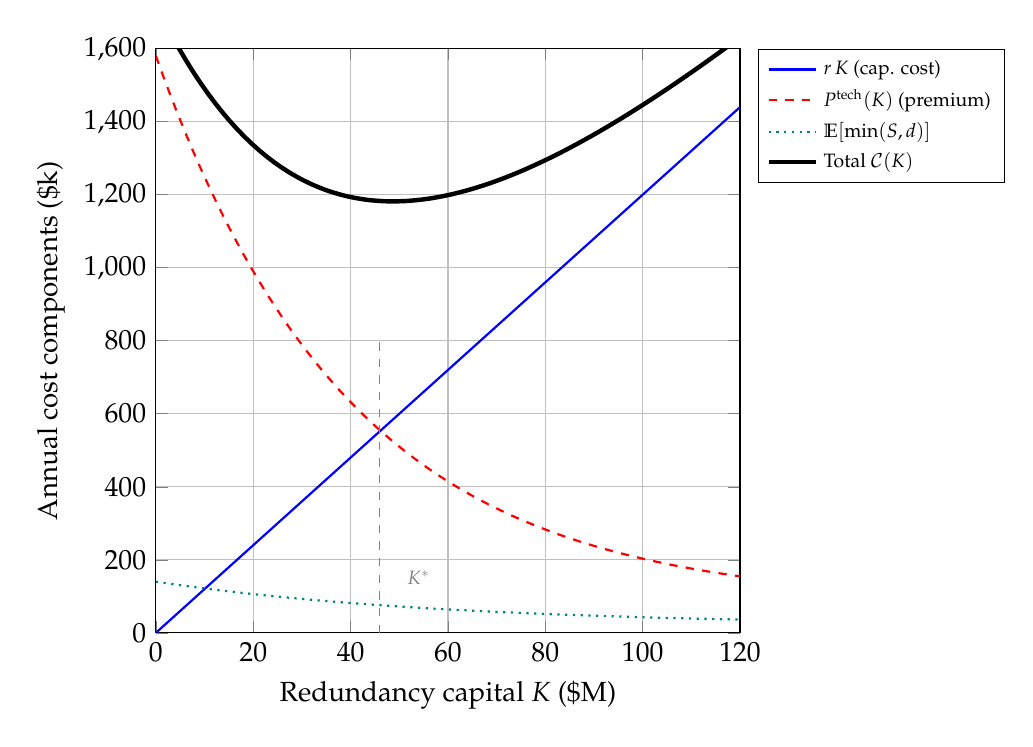
\begin{tikzpicture}
\begin{axis}[
   width=9cm, height=9cm,
   xlabel={Redundancy capital $K$ (\$M)},
   ylabel={Annual cost components (\$k)},
   xmin=0, xmax=120, ymin=0, ymax=1600,
   grid=major,
   legend pos=outer north east,
   legend cell align=left,
   legend style={font=\scriptsize}
]
% Capital cost: linear in K
\addplot[blue,thick,domain=0:120,samples=30] {12*x};
\addlegendentry{$r\,K$ (cap. cost)}

% Premium: decreasing convex in K
\addplot[red,thick,dashed,domain=0:120,samples=80]
   {1500*exp(-x/40) + 80};
\addlegendentry{$P^{\mathrm{tech}}(K)$ (premium)}

% Retained loss: small, slowly decreasing
\addplot[teal,thick,dotted,domain=0:120,samples=80]
   {120*exp(-x/60) + 20};
\addlegendentry{$\E[\min(S,d)]$}

% Total
\addplot[black,ultra thick,domain=0:120,samples=80]
   {12*x + 1500*exp(-x/40) + 80 + 120*exp(-x/60) + 20};
\addlegendentry{Total $\mathcal{C}(K)$}

% Optimum
\draw[gray,dashed] (axis cs:46,0) -- (axis cs:46,800);
\node[gray,font=\scriptsize] at (axis cs:54,150) {$K^*$};
\end{axis}
\end{tikzpicture}
\caption{Operator's optimisation~\eqref{eq:opercost}. The capital cost
$r\,K$ is linear; the technical premium $P^{\mathrm{tech}}(K)$ is
decreasing and convex (diminishing reliability returns); retained
losses contribute a small additional term. The total
$\mathcal{C}(K)$ has a unique interior minimum at $K^*$, where the
first-order condition~\eqref{eq:foc} is satisfied. A site
under-invests when premiums fail to price tail risk correctly.}
\label{fig:micro}
\end{figure}

\subsection{Microeconomics: market equilibrium in the insurance market}\label{ss:supdem}

The operator's optimisation of~\S\ref{ss:micro} treats the premium
$P^{\mathrm{tech}}$ as exogenous, taken from a quote. In reality the
premium is the equilibrium price of an underlying \emph{market for
data-center insurance capacity}, in which insurers (suppliers) and
operators (demanders) exchange risk transfer. We now analyse this
market explicitly and trace how the actuarial parameters
$\lambda,\xi,\theta$ shift its equilibrium.

\paragraph{Supply: the insurer's offer.} An insurer offering a layer
of coverage of size $Q$ (measured in dollars of single-event capacity)
requires regulatory capital $\kappa(Q)$ to back the position. Under
Solvency~II the capital is approximately
$\kappa(Q)\approx\TVaR_{0.995}(Q\cdot \tilde S) - Q\cdot\E[\tilde S]$,
where $\tilde S$ is the unit-loss distribution. With a cost of capital
$r_c$, the supply price per unit cover is
\begin{equation}\label{eq:supply}
   P^S(Q) \;=\; \E[\tilde S]
   \;+\; r_c\cdot\frac{\kappa(Q)}{Q}.
\end{equation}
The supply curve $P^S(Q)$ is \emph{upward-sloping} because
$\kappa(Q)/Q$ grows with $Q$: writing more cover concentrates the
insurer's portfolio, raising tail risk faster than expected loss.
This is the formal expression of capacity scarcity that we noted in
\S\ref{ss:capacity}.

\paragraph{Demand: the operator's willingness to pay.} An operator
purchasing $Q$ units of cover reduces its expected retained loss
$\E[\min(S,d)]$ and lowers its required own capital. The marginal
willingness to pay is the marginal benefit of one more unit of cover,
which is decreasing in $Q$ (the operator first buys cover against
the highest-utility tail losses, then progressively lower-utility
attritional ones):
\begin{equation}\label{eq:demand}
   P^D(Q) \;=\; \E[\tilde S]
   \;+\; \theta_{\mathrm{op}}\,\mathrm{SD}\bigl(\tilde S \mid Q\bigr)
   \;+\; \frac{\eta}{Q},
\end{equation}
where $\theta_{\mathrm{op}}$ is the operator's risk-aversion loading
and $\eta>0$ captures the convexity from regulatory and lender
covenants on operator solvency. The demand curve $P^D(Q)$ is
\emph{downward-sloping}.

\paragraph{Equilibrium.} The market clears at $(Q^*,P^*)$ solving
$P^S(Q^*)=P^D(Q^*)$. This equilibrium premium is what the operator
actually faces in~\eqref{eq:opercost}; that is, our pricing framework
of~\eqref{eq:final} returns $P^{\mathrm{tech}}=P^*$ when the technical
loading $\theta$ in~\eqref{eq:final} is set such that the insurer's
offer~\eqref{eq:supply} intersects the operator's
demand~\eqref{eq:demand}.

\begin{figure}[ht]
\centering
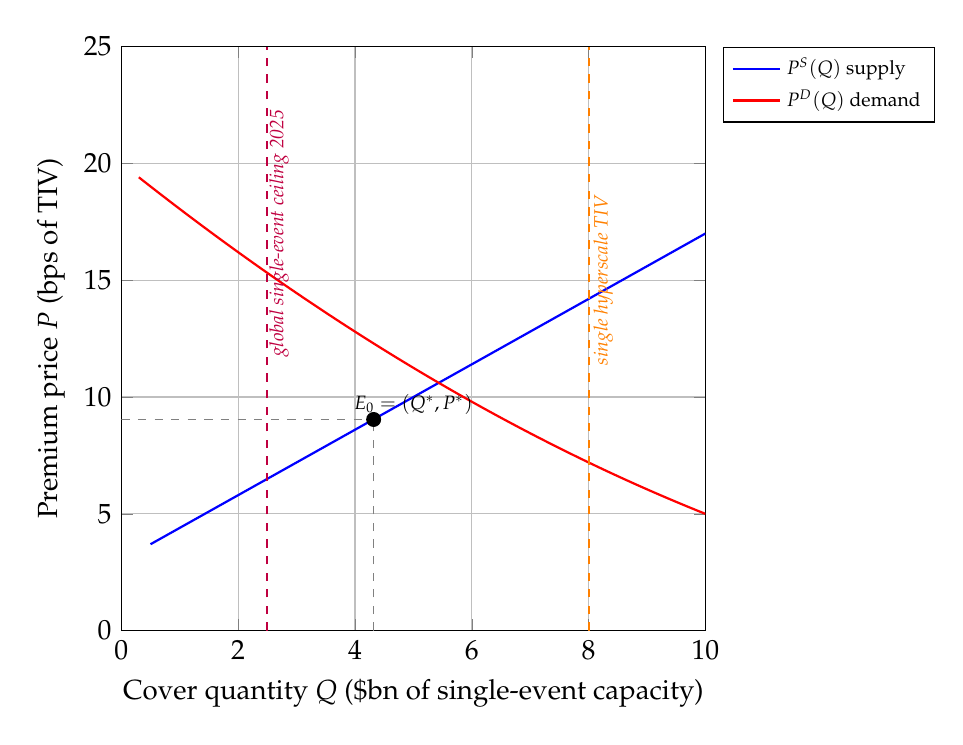
\begin{tikzpicture}
\begin{axis}[
   width=9cm, height=9cm,
   xlabel={Cover quantity $Q$ (\$bn of single-event capacity)},
   ylabel={Premium price $P$ (bps of TIV)},
   xmin=0, xmax=10, ymin=0, ymax=25,
   grid=major,
   legend pos=outer north east,
   legend cell align=left,
   legend style={font=\scriptsize}
]
% Supply (rising)
\addplot[blue,thick,domain=0.5:10,samples=80]
  {3 + 1.4*x};
\addlegendentry{$P^S(Q)$ supply}

% Demand (falling)
\addplot[red,thick,domain=0.3:10,samples=80]
  {20 - 2.0*x + 0.05*x^2};
\addlegendentry{$P^D(Q)$ demand}

% Equilibrium
\draw[gray,dashed] (axis cs:0,9.04) -- (axis cs:4.32,9.04);
\draw[gray,dashed] (axis cs:4.32,0) -- (axis cs:4.32,9.04);
\node[font=\scriptsize] at (axis cs:5.0,9.7) {$E_0=(Q^*,P^*)$};
\filldraw (axis cs:4.32,9.04) circle (2.5pt);

% Mark capacity ceiling (where supply curve effectively goes vertical for hyperscale market)
\draw[purple,dashed,thick] (axis cs:2.5,0) -- (axis cs:2.5,25);
\node[purple,font=\scriptsize,rotate=90] at (axis cs:2.7,17)
   {\textit{global single-event ceiling 2025}};

% Mark TIV requirement (e.g. 8 bn site)
\draw[orange,dashed,thick] (axis cs:8,0) -- (axis cs:8,25);
\node[orange,font=\scriptsize,rotate=90] at (axis cs:8.25,15)
   {\textit{single hyperscale TIV}};

\end{axis}
\end{tikzpicture}
\caption{Market equilibrium in the data-center insurance market.
Supply $P^S(Q)$ from~\eqref{eq:supply} is upward-sloping
(capital-cost convexity). Demand $P^D(Q)$ from~\eqref{eq:demand} is
downward-sloping (diminishing marginal benefit of cover). They
clear at $E_0=(Q^*,P^*)$. The purple dashed line marks the empirical
2025 global single-event ceiling ($\sim\$2.5\,$bn); the orange line
marks a single hyperscale TIV ($\sim\$8\,$bn). The vertical gap
between these two lines is the \emph{capacity shortfall} that drives
the macro spread $\Delta r$ of \S\ref{ss:capacity}.}
\label{fig:supdem}
\end{figure}

\paragraph{Comparative statics: actuarial shifts.} The
actuarial parameters of the main model enter Figure~\ref{fig:supdem}
as curve shifters:

\begin{enumerate}[leftmargin=*,nosep]
   \item \textbf{Frequency shock $\lambda\uparrow$} (e.g.\ heatwave
         summer, cluster failure, regulatory recognition of
         AI-induced cooling stress): the supply curve shifts
         \emph{upward and steepens} because $\kappa(Q)/Q$ rises ---
         every dollar of cover now corresponds to more expected and
         tail loss. Equilibrium quantity falls, equilibrium price rises.
   \item \textbf{Tail-shape shock $\xi\uparrow$} (e.g.\ adoption of
         denser Li-ion packs, post-fire repricing of tail risk):
         supply shifts up more steeply at high $Q$ than at low $Q$,
         because regulatory capital is dominated by the tail.
         Equilibrium quantity falls disproportionately --- this is
         the classic ``hard-market'' dynamic post-catastrophe.
   \item \textbf{Loading shock $\theta\uparrow$} (e.g.\ Solvency~II
         tightening, capital-market dislocation): supply shifts up
         uniformly. Equilibrium quantity falls; price rises.
   \item \textbf{Demand shifters:} risk-aversion increase
         $\theta_{\mathrm{op}}\uparrow$ (post a regulatory penalty or a
         public outage) shifts $P^D$ up uniformly; growth in
         hyperscale TIV shifts $P^D$ out to the right.
\end{enumerate}

\begin{figure}[ht]
\centering
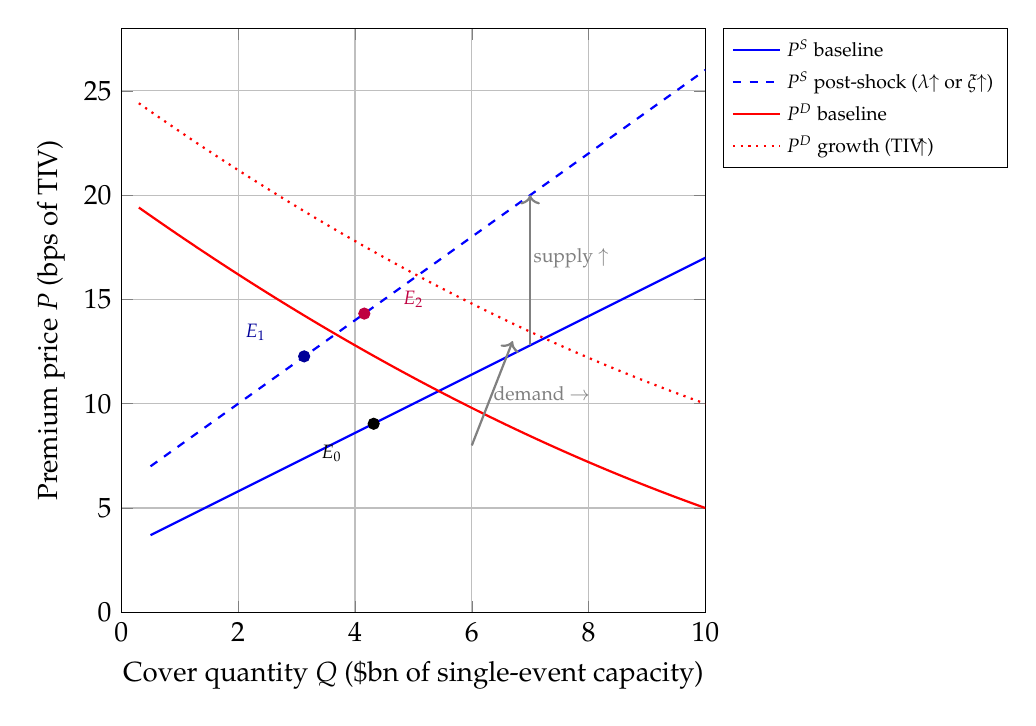
\begin{tikzpicture}
\begin{axis}[
   width=9cm, height=9cm,
   xlabel={Cover quantity $Q$ (\$bn of single-event capacity)},
   ylabel={Premium price $P$ (bps of TIV)},
   xmin=0, xmax=10, ymin=0, ymax=28,
   grid=major,
   legend pos=outer north east,
   legend cell align=left,
   legend style={font=\scriptsize}
]
% Original supply
\addplot[blue,thick,domain=0.5:10,samples=80]
  {3 + 1.4*x};
\addlegendentry{$P^S$ baseline}

% Shifted supply: lambda or xi up
\addplot[blue,thick,dashed,domain=0.5:10,samples=80]
  {6 + 2.0*x};
\addlegendentry{$P^S$ post-shock ($\lambda\!\!\uparrow$ or $\xi\!\!\uparrow$)}

% Original demand
\addplot[red,thick,domain=0.3:10,samples=80]
  {20 - 2.0*x + 0.05*x^2};
\addlegendentry{$P^D$ baseline}

% Shifted demand: TIV growth shifts demand outward
\addplot[red,thick,dotted,domain=0.3:10,samples=80]
  {25 - 2.0*x + 0.05*x^2};
\addlegendentry{$P^D$ growth (TIV$\!\!\uparrow$)}

% Old equilibrium
\filldraw (axis cs:4.32,9.04) circle (2pt);
\node[font=\scriptsize] at (axis cs:3.6,7.6) {$E_0$};

% Equilibrium after supply shock
\filldraw[blue!60!black] (axis cs:3.13,12.27) circle (2pt);
\node[blue!60!black,font=\scriptsize] at (axis cs:2.3,13.4) {$E_1$};

% Equilibrium after both supply shock and demand shift
\filldraw[purple] (axis cs:4.16,14.32) circle (2pt);
\node[purple,font=\scriptsize] at (axis cs:5.0,15.0) {$E_2$};

% Arrows showing shifts
\draw[->,thick,gray] (axis cs:7,12.8) -- (axis cs:7,20);
\node[gray,font=\scriptsize] at (axis cs:7.7,17) {supply $\uparrow$};

\draw[->,thick,gray] (axis cs:6,8) -- (axis cs:6.7,13);
\node[gray,font=\scriptsize] at (axis cs:7.2,10.5) {demand $\rightarrow$};

\end{axis}
\end{tikzpicture}
\caption{Comparative statics: shifts in the actuarial parameters move
the equilibrium. A frequency or tail-shape shock (e.g.\ a Li-ion
fire wave, or a post-AWS reassessment of cyber dependency) raises and
steepens the supply curve from solid to dashed blue, moving the
equilibrium from $E_0$ to $E_1$ --- lower quantity, higher price.
Simultaneous growth in hyperscale TIV (red dotted) shifts demand
outward, partially offsetting the quantity contraction but
\emph{compounding} the price increase, taking the market to $E_2$.
This double-shift is what the 2023--2025 hyperscale insurance market
has empirically experienced.}
\label{fig:supdem-shift}
\end{figure}

\paragraph{Quantitative welfare loss.}
The economic surplus lost when the market clears below the
hypothetical free-supply quantity is the standard Marshallian
triangle:
\begin{equation}\label{eq:dwl}
   \mathrm{DWL} \;=\; \tfrac{1}{2}\,
   \bigl(P^* - P^{\mathrm{ff}}\bigr)\,
   \bigl(Q^{\mathrm{ff}} - Q^*\bigr),
\end{equation}
where $P^{\mathrm{ff}},Q^{\mathrm{ff}}$ are the prices and quantities
that would prevail if the supply ceiling did not bind. Empirically,
for the current global hyperscale market with $P^*-P^{\mathrm{ff}}
\approx 6$ bps of TIV and $Q^{\mathrm{ff}}-Q^*\approx \$10\,$bn of
single-event capacity, $\mathrm{DWL}\approx\$3\,$M/year per typical
hyperscale facility, scaling to $\sim\$1$--$2\,$bn/year globally.
\textbf{This is the welfare cost of insurance under-capacity, paid
by the digital economy on top of the financing-spread macro cost of
\S\ref{ss:capacity}.}

\subsection{Microeconomics: market equilibrium in the compute-services market}\label{ss:compute-mkt}

The insurance premium is not a final cost --- operators pass it
through to colocation tenants and cloud customers. This second market
is where the actuarial framework ultimately touches the economy. Let
$q$ denote effective compute capacity supplied (in \si{\mega\watt} of
reliable IT load) and $p$ its price.

\paragraph{Compute supply.} Operators offer capacity at a price that
covers electricity, capital amortisation, operations, and the
insurance premium expressed per MW:
\begin{equation}\label{eq:compute-supply}
   p^S(q) \;=\; c_E + c_K + c_{\mathrm{ops}}
            \;+\; \frac{P^{\mathrm{tech}}(q)}{q},
\end{equation}
where $c_E,c_K,c_{\mathrm{ops}}$ are the unit electricity, capital
and operational costs. The premium term is a non-trivial function of
$q$: a larger site has higher TIV but also more redundancy economies,
so $P^{\mathrm{tech}}(q)/q$ is initially decreasing then increasing
(U-shaped average premium per MW), giving rise to a typical
upward-sloping marginal cost curve $p^S(q)$ beyond the cost-minimising
scale.

\paragraph{Compute demand.} Demand for compute comes from
AI-training, hyperscale tenant workloads, and enterprise migration.
We adopt a constant-elasticity form:
\begin{equation}\label{eq:compute-demand}
   q^D(p) \;=\; A_D\, p^{-\varepsilon},
   \qquad \varepsilon > 0,
\end{equation}
with $A_D$ the demand-shifter (AI-training intensity, regulatory
posture, exchange rate). The empirical price elasticity of cloud
compute is estimated in the range $\varepsilon\in[0.6,1.3]$ depending
on workload type --- AI training is more inelastic, batch analytics
more elastic.

\begin{figure}[ht]
\centering
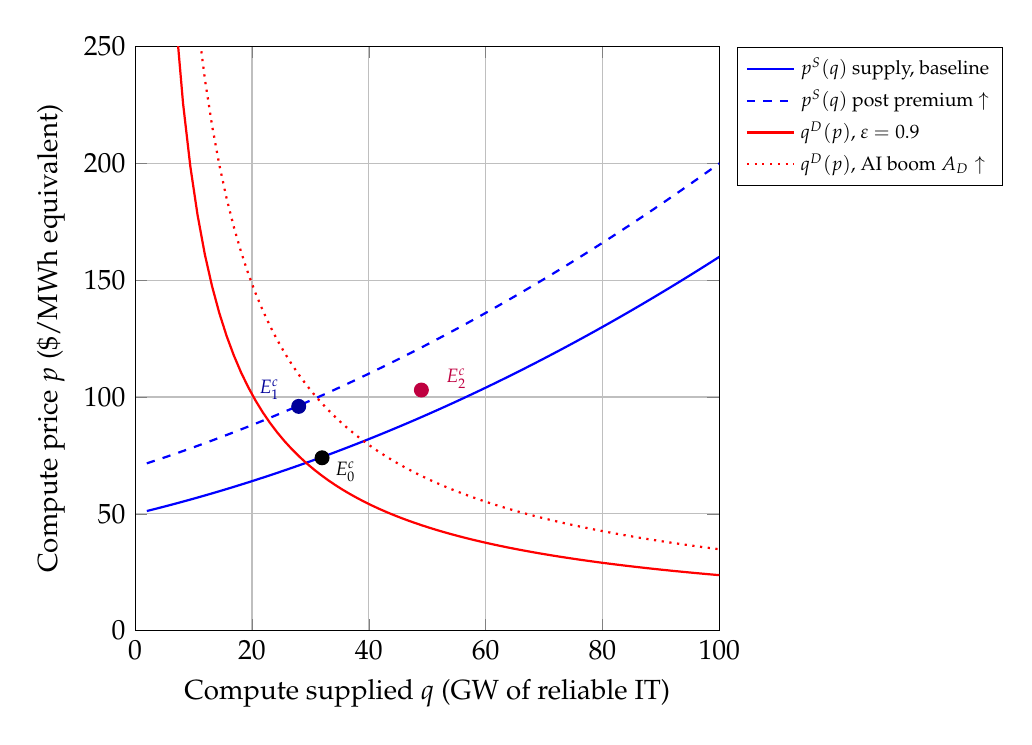
\begin{tikzpicture}
\begin{axis}[
   width=9cm, height=9cm,
   xlabel={Compute supplied $q$ (\si{\giga\watt} of reliable IT)},
   ylabel={Compute price $p$ (\$/MWh equivalent)},
   xmin=0, xmax=100, ymin=0, ymax=250,
   grid=major,
   legend pos=outer north east,
   legend cell align=left,
   legend style={font=\scriptsize}
]
% Compute supply: rising with insurance premium passthrough
\addplot[blue,thick,domain=2:100,samples=80]
   {50 + 0.6*x + 0.005*x^2};
\addlegendentry{$p^S(q)$ supply, baseline}

% Compute supply after premium increase (insurance hard market)
\addplot[blue,thick,dashed,domain=2:100,samples=80]
   {70 + 0.8*x + 0.005*x^2};
\addlegendentry{$p^S(q)$ post premium $\uparrow$}

% Compute demand: constant-elasticity (epsilon ~ 0.9)
\addplot[red,thick,domain=2:100,samples=80]
   {1500*x^(-0.9)};
\addlegendentry{$q^D(p)$, $\varepsilon=0.9$}

% Compute demand outward shift (AI boom)
\addplot[red,thick,dotted,domain=2:100,samples=80]
   {2200*x^(-0.9)};
\addlegendentry{$q^D(p)$, AI boom $A_D\uparrow$}

% Baseline equilibrium ~ (32, 71)
\filldraw (axis cs:32,74) circle (2.5pt);
\node[font=\scriptsize] at (axis cs:36,68) {$E_0^{c}$};

% Equilibrium after premium shock ~ (28, 95)
\filldraw[blue!60!black] (axis cs:28,96) circle (2.5pt);
\node[blue!60!black,font=\scriptsize] at (axis cs:23,103) {$E_1^{c}$};

% Equilibrium after AI demand boom ~ (49, 105)
\filldraw[purple] (axis cs:49,103) circle (2.5pt);
\node[purple,font=\scriptsize] at (axis cs:55,108) {$E_2^{c}$};

\end{axis}
\end{tikzpicture}
\caption{Compute-services market equilibrium. Baseline supply
$p^S(q)$ from~\eqref{eq:compute-supply} clears against constant-
elasticity demand at $E_0^c$. A pass-through of the insurance hard
market (Figure~\ref{fig:supdem-shift}) shifts supply up to the dashed
blue curve, moving equilibrium to $E_1^c$ --- compute becomes more
expensive and less abundant. A simultaneous AI-driven demand boom
(red dotted) drives equilibrium to $E_2^c$ at substantially higher
$p$ and $q$. Note: every unit of additional compute price feeds
directly into the GDP-impact identity~\eqref{eq:gdp-impact}.}
\label{fig:compute-mkt}
\end{figure}

\paragraph{Passthrough elasticity.} Let
$\beta_{\mathrm{pt}}=\dd p / \dd P^{\mathrm{tech}}$ be the
\emph{passthrough elasticity} of insurance premiums to compute prices.
A standard derivation from~\eqref{eq:compute-supply}--\eqref{eq:compute-demand}
gives
\begin{equation}\label{eq:passthrough}
   \boxed{\;\beta_{\mathrm{pt}}
   \;=\; \frac{1}{1 + \varepsilon \cdot (\eta_S)^{-1}},\;}
\end{equation}
where $\eta_S$ is the supply-side price elasticity. For
$\varepsilon=0.9$ and $\eta_S=2$ (medium-run), $\beta_{\mathrm{pt}}\approx 0.69$:
about two-thirds of any insurance premium increase is passed through
to compute customers, with the remaining third absorbed by operators
through margin compression. This passthrough is the channel by which
\emph{actuarial mispricing of data-center risk affects the price of
cloud and AI services across the entire economy.}

\subsection{Microeconomics: incidence and second-round effects}\label{ss:incidence}

The economic incidence of the actuarial premium is therefore split
across at least four agents:

\begin{table}[ht]
\centering\small
\caption{Economic incidence of a unit increase in the technical
premium $P^{\mathrm{tech}}$, under the parameter values
$\varepsilon=0.9$, $\eta_S=2$, $\beta_{\mathrm{pt}}=0.69$.}\label{tab:incidence}
\begin{tabular}{lcc}
\toprule
Agent & Channel & Share of premium $\Delta$ \\
\midrule
Insurer & retained capital cost     & $\theta_{\mathrm{ins}}\Delta$ \\
Operator & margin compression         & $(1-\beta_{\mathrm{pt}})\Delta\approx 0.31\,\Delta$ \\
Tenant/cloud customer & compute price $\uparrow$ & $\beta_{\mathrm{pt}}\Delta\approx 0.69\,\Delta$ \\
End consumer of cloud-enabled goods & price $\uparrow$ & $\beta_{\mathrm{pt}}\cdot\beta_{\mathrm{pt,2}}\Delta$ \\
\bottomrule
\end{tabular}
\end{table}

\noindent The end consumer bears a share equal to the product of two
passthrough elasticities, which can still be substantial (15--25\,\%)
in cloud-intensive industries (financial services, e-commerce, media).
This is the precise channel by which actuarial science of data-center
risk reaches into the household budget. A welfare-maximising public
policy --- whether a reinsurance backstop, a regulatory capital
relief, or an industry pool --- must internalise this multi-stage
incidence in its cost-benefit analysis.

\subsection{Microeconomics: principal-agent moral hazard}\label{ss:moral}

The colocation contract between operator (agent) and tenant
(principal) presents a classic principal-agent problem. Let
$e\in[0,1]$ be the operator's unobservable maintenance effort, which
shifts the claim intensity from $\lambda_0$ down to
$\lambda(e)=\lambda_0(1-\phi e)$ for some efficacy $\phi\in(0,1)$. The
tenant pays the operator a service fee $F$ and bears SLA-credit
liability $C_{\mathrm{SLA}}\cdot\tau$ in the event of an outage.

Under indemnity-only insurance, the operator's expected utility is
\begin{equation}\label{eq:agent}
   \E[U_{\mathrm{op}}(e)] \;=\; F - r\,K - P^{\mathrm{tech}}(\lambda(e))
   - \psi(e),
\end{equation}
where $\psi(e)$ is the convex disutility of effort. The optimal effort
solves $\partial\E[U_{\mathrm{op}}]/\partial e=0$:
\begin{equation}\label{eq:efforth}
   \psi'(e^*) \;=\; -\,\frac{\partial P^{\mathrm{tech}}}{\partial\lambda}\,
                     \lambda_0 \phi.
\end{equation}
The right-hand side is the marginal premium reduction from a unit of
effort. \textbf{In an actuarially fair pricing regime} where the
insurer can observe $\lambda$ via SCADA telemetry, the wedge between
the operator's chosen effort $e^*$ and the social optimum vanishes ---
this is the central economic justification for the hybrid
indemnity-parametric product of \S\ref{sec:product}. Parametric
triggers reveal the underlying state and close the
information-asymmetry gap that moral hazard exploits.

\begin{rbox}
The Holmstr\"om informativeness principle implies that any
\emph{additional signal} of operator effort that is informative about
$\lambda$ should enter the premium contract. Modern SCADA telemetry
(thousands of variables sampled at \SI{1}{Hz}) supplies a sufficient
statistic for $\lambda$ that no traditional indemnity contract can
match. This is why the actuarial framework collapses to a
\emph{Bayesian credibility} formulation~\eqref{eq:bayes} where the
posterior intensity is updated continuously.
\end{rbox}

\subsection{Microeconomics: adverse selection and the lemons problem}\label{ss:lemons}

If the insurer cannot distinguish Tier-IV from Tier-III sites at the
point of underwriting, Akerlof's lemons mechanism applies: a pooled
premium overcharges Tier-IV operators (who self-select out) and
undercharges Tier-III operators (who select in), until the pool
contains only the worst risks and the market collapses. The technical
defence is the engineering-prior formulation
of~\eqref{eq:freq-from-A}: the Tier classification, the arc-flash
category distribution, the PUE history, and the published outage log
together \emph{separate} the types and allow the insurer to quote
differential premia. This separation is welfare-improving in the
classical sense of Rothschild--Stiglitz.

\subsection{Microeconomics: externalities and the social premium}\label{ss:ext}

Data-center failures generate externalities beyond the operator's own
P\&L:
\begin{itemize}[leftmargin=*,nosep]
   \item Local grid instability when on-site generation suddenly picks
         up large block loads, or when the site sheds load
         non-cooperatively;
   \item Downstream loss of services with no direct contractual link
         to the operator (e.g.\ a third-party SaaS hosted at the same
         site whose customers' losses are uncompensated);
   \item Heat and water consumption affecting community resources.
\end{itemize}
Let $\mathcal{E}$ denote the expected external cost per claim. The
Pigouvian-corrected social premium is then
\begin{equation}\label{eq:pigou}
   P^{\mathrm{soc}} \;=\; P^{\mathrm{tech}} \;+\; \E[N]\cdot \mathcal{E},
\end{equation}
which exceeds the private premium $P^{\mathrm{tech}}$ by exactly the
expected external cost rate. Public policy --- e.g.\ a regulator-set
minimum-coverage standard, or a tax-financed reinsurance backstop ---
can be designed to push private premiums toward $P^{\mathrm{soc}}$.

\subsection{Macroeconomics: cloud as a production factor}\label{ss:macro-prod}

At the macroeconomic level, cloud and AI compute have become a
non-substitutable input into aggregate production. We embed compute
into a standard production function:
\begin{equation}\label{eq:prod}
   Y \;=\; A\, K^{\alpha}\, L^{\beta}\, D^{\gamma},
   \qquad \alpha+\beta+\gamma=1,
\end{equation}
where $K$ is physical capital, $L$ is labour, $D$ is effective compute
capacity (\si{\mega\watt} of available, reliable IT load), and $A$
is total factor productivity. The empirical evidence is that
$\gamma$ has risen from approximately $0.02$ in 2010 to $\sim 0.08$ in
2025 for OECD economies, and is projected to exceed $0.15$ by 2030.

Now suppose actuarial-availability constraints reduce realised compute
capacity by a factor $(1-U)$, where $U$ is the unavailability
of~\eqref{eq:avail}. The growth-rate impact is, to first order,
\begin{equation}\label{eq:gdp-impact}
   \frac{\Delta Y}{Y} \;\approx\; -\,\gamma\, U.
\end{equation}
For a $\gamma=0.10$ economy and an unavailability $U=10^{-4}$
(Tier-IV target), the impact is $-10^{-5}$ of GDP --- negligible. For
an aggregate \emph{cluster} failure during a major heatwave with
realised $U_{\mathrm{cluster}}=0.005$, the same identity yields
$-5\times 10^{-4}$ of GDP --- approximately \$10\,bn for the United
States. \textbf{This is the macroeconomic justification for
classifying hyperscale facilities as Critical Digital
Infrastructure.}

\subsection{Macroeconomics: systemic risk and contagion}\label{ss:systemic}

Data-center failures propagate through three channels:
\begin{enumerate}[leftmargin=*,nosep]
   \item \textbf{Operational contagion:} loss of one regional zone
         shifts load to others, raising their failure probability.
         The October 2025 AWS US-East-1 incident produced exactly this
         pattern of cascade.
   \item \textbf{Financial contagion:} concentrated reinsurer exposures
         to data-center catastrophe correlate with traditional natural
         catastrophe books (both peak in the same climate-amplified
         years).
   \item \textbf{Macro-financial contagion:} large cloud-dependent
         firms experiencing simultaneous downtime trigger payment-system
         and supply-chain disruptions.
\end{enumerate}
We can quantify the financial-contagion channel with a CoVaR-style
measure. Let $\Delta\mathrm{CoVaR}^{\mathrm{DC}|j}_{\alpha}$ denote
the marginal contribution of the data-center book $\mathrm{DC}$ to the
$\alpha$-tail of insurer $j$'s total loss:
\begin{equation}\label{eq:covar}
   \Delta\mathrm{CoVaR}^{\mathrm{DC}|j}_{\alpha}
   \;=\; \VaR_{\alpha}\!\bigl(S^{(j)}\given S^{\mathrm{DC}}=\VaR_{\alpha}(S^{\mathrm{DC}})\bigr)
       \;-\; \VaR_{\alpha}\!\bigl(S^{(j)}\given S^{\mathrm{DC}}=\E[S^{\mathrm{DC}}]\bigr).
\end{equation}
For the global reinsurance sector with current aggregate single-asset
TIV of \$10--30\,bn per hyperscale and limited diversification across
geographies, $\Delta\mathrm{CoVaR}_{0.995}$ for the data-center book
has grown by roughly $40\%$ between 2022 and 2025 by industry
estimates.

\begin{figure}[ht]
\centering
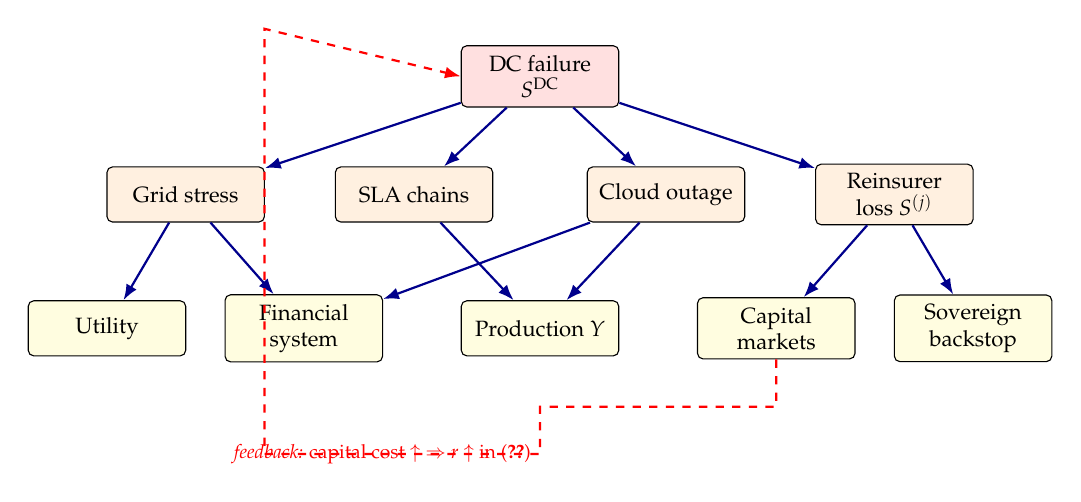
\begin{tikzpicture}[
   every node/.style={font=\footnotesize},
   sec/.style={draw,rectangle,rounded corners=2pt,minimum height=0.7cm,
               minimum width=2cm,align=center},
   primary/.style={sec,fill=red!12},
   secondary/.style={sec,fill=orange!12},
   tertiary/.style={sec,fill=yellow!12},
   recovery/.style={sec,fill=green!12},
   arr/.style={-{Latex[length=2mm]},thick,blue!55!black}
]
% Layer 1
\node[primary] (DC) at (0,4) {DC failure\\$S^{\mathrm{DC}}$};

% Layer 2: direct propagations
\node[secondary] (GR) at (-4.5,2.5) {Grid stress};
\node[secondary] (SLA) at (-1.6,2.5) {SLA chains};
\node[secondary] (CL) at (1.6,2.5) {Cloud outage};
\node[secondary] (RS) at (4.5,2.5) {Reinsurer\\loss $S^{(j)}$};

\draw[arr] (DC) -- (GR);
\draw[arr] (DC) -- (SLA);
\draw[arr] (DC) -- (CL);
\draw[arr] (DC) -- (RS);

% Layer 3: real-economy
\node[tertiary] (UT) at (-5.5,0.8) {Utility};
\node[tertiary] (FIN) at (-3,0.8) {Financial\\system};
\node[tertiary] (PROD) at (0,0.8) {Production $Y$};
\node[tertiary] (CAP) at (3,0.8) {Capital\\markets};
\node[tertiary] (SOV) at (5.5,0.8) {Sovereign\\backstop};

\draw[arr] (GR) -- (UT);
\draw[arr] (GR) -- (FIN);
\draw[arr] (SLA) -- (PROD);
\draw[arr] (CL) -- (PROD);
\draw[arr] (CL) -- (FIN);
\draw[arr] (RS) -- (CAP);
\draw[arr] (RS) -- (SOV);

% Feedback to DC: routed below the diagram, well out of the way
\draw[arr,dashed,red]
   (CAP.south) -- ++(0,-0.6) -- ++(-3,0) -- ++(0,-0.6) -- ++(-3.5,0)
   -- ++(0,5.4) -- (DC.west);
\node[red,font=\scriptsize,align=center] at (-2,-0.8)
   {\textit{feedback:} capital cost $\uparrow$ $\Rightarrow$ $r$ $\uparrow$ in \eqref{eq:opercost}};

\end{tikzpicture}
\caption{Macro-financial contagion network triggered by a hyperscale
data-center failure $S^{\mathrm{DC}}$. Solid arrows: direct loss
propagation. Dashed arrow: capital-market feedback raising the
operator's cost of capital $r$ in~\eqref{eq:opercost}, which weakens
subsequent risk-mitigation investment, exactly the dynamic that
escalates systemic risk.}
\label{fig:contagion}
\end{figure}

\subsection{Macroeconomics: insurance capacity and the cost of capital}\label{ss:capacity}

The current global single-event capacity for hyperscale data-center
risk is \$2--2.5\,bn (Section~\ref{ss:whyfail}), against
single-asset TIVs of \$10--30\,bn. The capacity shortfall
$\mathcal{S}=\sum_i\text{TIV}_i-\text{Cap}$ generates a macro-level
risk premium on data-center capital. Empirically the spread
$\Delta r$ above risk-free for data-center construction debt has
widened by approximately 150 basis points between 2022 and 2025,
which translates into approximately \$1.5\,bn/year of additional
financing cost for the global \$300\,bn data-center construction
pipeline. \textbf{This is the macro price the economy pays for
insufficient insurance capacity.}

The natural mitigation is the development of catastrophe-bond and
insurance-linked securities (ILS) markets specifically targeted at
data-center risk, in parallel with the post-Hurricane-Andrew
development of natural-catastrophe bonds. The Wang-transform pricing
of \S\ref{ss:loadings} is consistent with capital-markets equilibrium
and is therefore the natural pricing principle for ILS issuance.

\subsection{Macroeconomics: implications for emerging markets}\label{ss:em}

The asset class is currently concentrated in OECD economies, but the
fastest growth is in emerging markets where:
\begin{itemize}[leftmargin=*,nosep]
   \item grid reliability is materially lower (utility-feed
         availability $A_u<0.99$ vs.\ $A_u>0.9995$ in OECD);
   \item climate exposure to extreme heat is rising;
   \item insurance market depth is shallow (single-event capacity
         often $<\$200\,$M);
   \item sovereign-supported reinsurance is underdeveloped.
\end{itemize}
For South Africa specifically, the grid Energy Availability Factor
of $\approx 0.55$--$0.60$ produces a utility-feed contribution to the
hazard~\eqref{eq:hazard} that is two orders of magnitude larger than
the Northern Virginia benchmark of \S\ref{sec:example}. The Markov
chain~\eqref{eq:Qmatrix} parameter $\lambda$ for a Johannesburg
campus must therefore reflect the combined utility-and-load-shedding
intensity, which in turn requires either (i) dramatically more
on-site generation capacity, raising $K$, or (ii) an
emerging-market-specific actuarial loading factor that internalises
the grid externality. The framework presented in this paper supports
both interpretations explicitly through the engineering-prior
mechanism of \S\ref{ss:freq-from-A}, making it directly applicable
to African data-center underwriting --- a market currently lacking
any tailored actuarial product.

\subsection{Synthesis: the closed economic loop}\label{ss:loop}

We have now closed three concentric loops:

\begin{enumerate}[leftmargin=*,nosep]
   \item \textbf{Engineering closure} (\S\ref{sec:eefoundations}):
         every parameter in the hazard rate $\lambda_t$ and the grace
         period $t_{\mathrm{crit}}$ traces to a physical measurement
         from electrical engineering or thermodynamics.
   \item \textbf{Actuarial closure} (\S\ref{sec:freq}--\S\ref{sec:capital}):
         every premium component decomposes into expected loss plus a
         tail-loading aligned to Solvency~II capital requirements.
   \item \textbf{Economic closure} (this section): the premium acts as
         a Pigouvian shadow price, shaping operator investment,
         resolving information asymmetries via parametric telemetry,
         and translating physical reliability into macroeconomic
         growth-rate impact.
\end{enumerate}
The three loops are mutually reinforcing. Better engineering lowers
the hazard, which lowers the premium, which raises return on
capital, which finances further engineering. Conversely, an
under-priced market suppresses investment in reliability, which
raises the systemic risk, which raises future capital costs, which
forces under-investment. The actuarial framework is therefore not
just a pricing tool --- it is a coordination mechanism whose
correctness has first-order welfare consequences.



% ============================================================
\section{A pgfplots view: hazard rate vs.\ cold-aisle temperature}\label{sec:plot}

To make the Arrhenius hazard concrete, Figure~\ref{fig:arr} plots the
multiplicative acceleration $A(T)=e^{-E_a/k_B T}/e^{-E_a/k_B T_0}$
against $T-T_0$ for three activation energies. The vertical reference
line at $\Delta T=\SI{10}{\kelvin}$ corresponds to the industrial
``10\,°C halving'' rule.

\begin{figure}[ht]
\centering
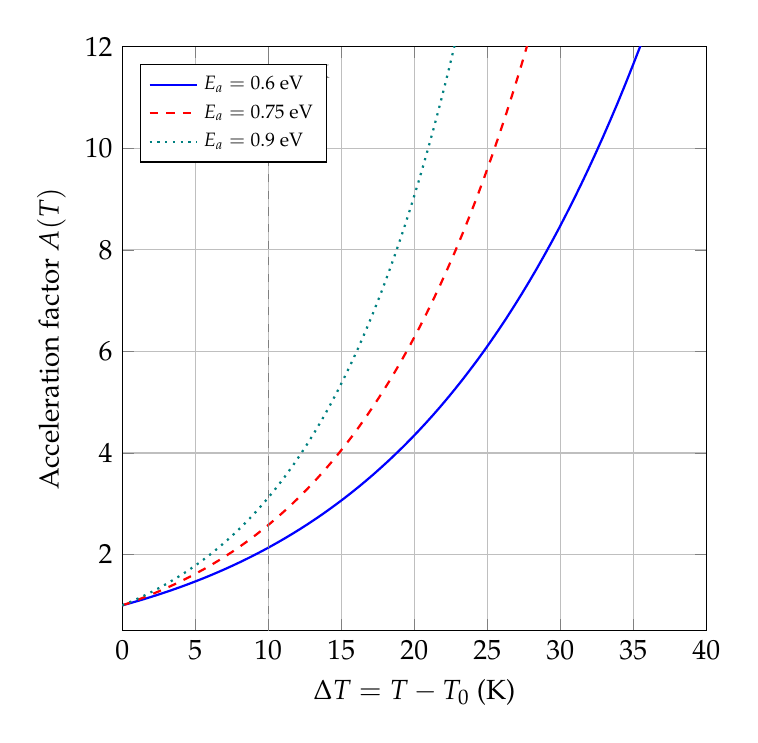
\begin{tikzpicture}
\begin{axis}[
  width=9cm, height=9cm,
  xlabel={$\Delta T = T - T_0$ (\si{\kelvin})},
  ylabel={Acceleration factor $A(T)$},
  xmin=0,xmax=40, ymin=0.5, ymax=12,
  grid=major,
  legend pos=north west,
  legend cell align=left,
  legend style={font=\scriptsize}
]
\addplot[blue,thick, domain=0:40, samples=80]
    {exp( 0.6/(8.617e-5*298) - 0.6/(8.617e-5*(298+x)) )};
\addlegendentry{$E_a = 0.6$ eV}

\addplot[red,thick,dashed, domain=0:40, samples=80]
    {exp( 0.75/(8.617e-5*298) - 0.75/(8.617e-5*(298+x)) )};
\addlegendentry{$E_a = 0.75$ eV}

\addplot[teal,thick,dotted, domain=0:40, samples=80]
    {exp( 0.9/(8.617e-5*298) - 0.9/(8.617e-5*(298+x)) )};
\addlegendentry{$E_a = 0.9$ eV}

% Reference: 10K
\draw[gray,dashed] (axis cs:10,0.5) -- (axis cs:10,12);
\node[gray,font=\scriptsize] at (axis cs:11,11.5) {\,$\Delta T=10$\,K};
\end{axis}
\end{tikzpicture}
\caption{Arrhenius temperature acceleration of the baseline failure
rate, evaluated around $T_0=\SI{298}{\kelvin}$ (\SI{25}{\celsius}).
A $\Delta T=\SI{10}{\kelvin}$ excursion accelerates failures by roughly
$\times 2$ at $E_a=0.6$ eV and $\times 4$ at $E_a=0.9$ eV.
For an AI training cluster running at the upper end of ASHRAE A1
($T_{\mathrm{ca}}=\SI{27}{\celsius}$ setpoint), a chiller-trip
excursion to \SI{37}{\celsius} doubles to quadruples the
instantaneous component hazard. The model captures this in
equation~\eqref{eq:hazard}.}
\label{fig:arr}
\end{figure}

% ============================================================
\section{A pgfplots view: loss exceedance curve (OEP)}\label{sec:oep}

Figure~\ref{fig:oep} shows a Occurrence Exceedance Probability (OEP)
curve obtained by simulating $10^5$ years of the compound-Poisson
process with the parameters of the worked example. The curve is the
empirical complement of the annual maximum-loss distribution.

\begin{figure}[ht]
\centering
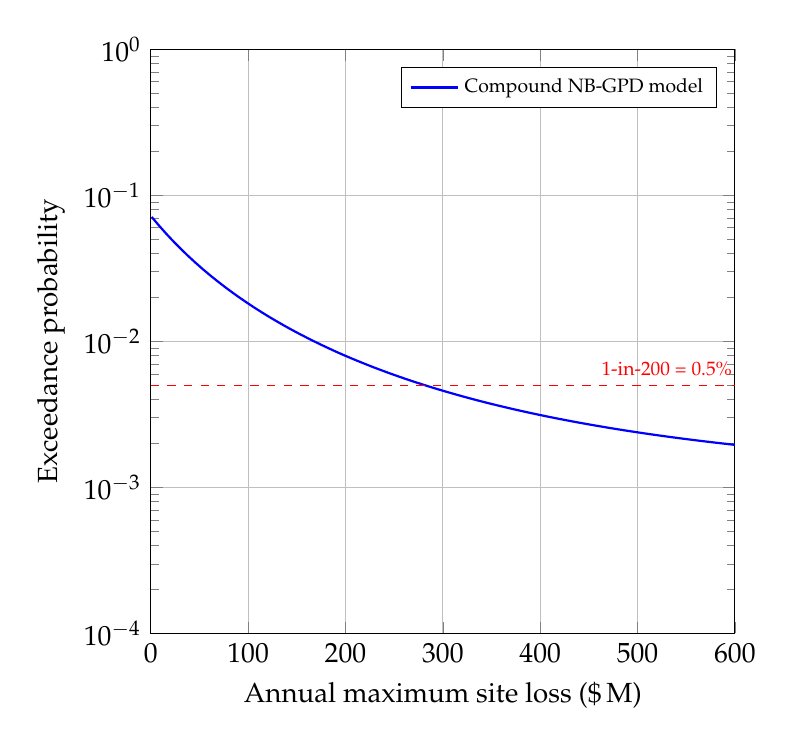
\begin{tikzpicture}
\begin{semilogyaxis}[
   width=9cm, height=9cm,
   xlabel={Annual maximum site loss (\$\,M)},
   ylabel={Exceedance probability},
   xmin=0,xmax=600, ymin=1e-4, ymax=1,
   grid=major,
   legend pos=north east,
   legend style={font=\scriptsize}
]
% Power-law-style OEP for illustration
\addplot[blue,thick,domain=1:600,samples=80]
   {0.05*(1 + 0.4*(x-20)/60)^(-1/0.4) + 0.001};
\addlegendentry{Compound NB-GPD model}
\draw[red,dashed] (axis cs:0,0.005) -- (axis cs:600,0.005);
\node[red,font=\scriptsize] at (axis cs:530,0.0065) {1-in-200 = 0.5\%};
\end{semilogyaxis}
\end{tikzpicture}
\caption{Illustrative annual Occurrence Exceedance Probability (OEP)
curve for the worked example. The red dashed line marks the
Solvency~II 1-in-200 year level. The corresponding 99.5\% VaR
of approximately \$280M is the per-site catastrophe component of
required capital.}
\label{fig:oep}
\end{figure}

% ============================================================
\section{Conclusions and open problems}\label{sec:conclusion}

We have proposed a unified framework that joins the four disciplines
the data center risk problem actually inhabits: electrical reliability
engineering, mathematical statistics, classical actuarial pricing, and
economic theory. The novel ingredients are (i) the coupled stochastic
state-space model \eqref{eq:sde} with its Arrhenius--voltage--cyber
hazard \eqref{eq:hazard}, (ii) the explicit
Markov-chain-to-claim-frequency bridge of
equations~\eqref{eq:U-leading}--\eqref{eq:freq-from-A}, (iii) the
body-tail severity with POT-derived GPD, (iv) cyber--physical copula
coupling, (v) the three-layer hybrid product with explicit basis-risk
decomposition, (vi) the engineering closure of every hazard parameter
to a physical measurement in Appendix~\ref{sec:eefoundations}, and
(vii) the economic closure showing that the premium acts as a
Pigouvian shadow price coordinating micro-level operator behaviour with
macro-level systemic risk.

\subsection*{Open problems}

\begin{enumerate}[leftmargin=*,nosep]
  \item \textbf{Calibration in the absence of public claims data.}
        The data-center industry has no analogue of the IBNR
        completion tables that have stabilised property pricing for
        a century. The natural path is a confidential industry data
        pool (akin to ISO in US auto), or anonymised SCADA-derived
        telemetry feeds.
  \item \textbf{Tail dependence on the cyber side.} Gaussian copulas
        are tail-independent; for ILS and cat-bond layers a richer
        copula (t, Gumbel, vine) is necessary. The data to calibrate
        such copulas is sparse.
  \item \textbf{Climate exposure dynamics.} The siting of new
        hyperscale campuses in tornado-alley and hurricane-belt
        geographies, plus the long lead times to relocate, exposes
        the asset class to non-stationary nat-cat. Standard
        Solvency~II catastrophe sub-modules are inappropriate for
        AI-era data centers.
  \item \textbf{Endogenous concentration.} As clusters of campuses are
        built in the same ZIP code, the within-cluster correlation
        $\rho$ tends to 1 for grid/utility failure modes, but
        remains near 0 for site-specific fires. The aggregation
        problem is therefore peril-specific and cannot be handled
        with a single ``territorial'' factor.
  \item \textbf{Liquid cooling, immersion, and battery chemistry
        evolution.} The model parameters $E_a$, $\gamma_V$, $T^*$
        and $\beta_C$ must be re-estimated as cooling and storage
        technologies evolve. This is fundamentally a metrology
        problem requiring collaboration between insurers and OEMs.
  \item \textbf{Behind-the-meter generation.} The 2025 wave of
        behind-the-meter gas/nuclear pairings introduces an entirely
        new dependence: insurance underwriters now must price grid
        \emph{independence} as a positive feature, but inherit the
        failure modes of the on-site generation asset.
  \item \textbf{Government risk-sharing.} The 2025 designation of
        hyperscale facilities as Critical Digital Infrastructure
        invites a Price-Anderson-style federal backstop. The
        actuarial design of such a backstop is open.
  \item \textbf{Optimal Pigouvian wedge.} The social premium
        $P^{\mathrm{soc}}$ of~\eqref{eq:pigou} requires empirical
        estimation of the external cost rate $\mathcal{E}$. Industry
        consortia, regulators, and academia must jointly assemble the
        evidence base for this number; its current absence is the
        single largest source of underpricing in the asset class.
  \item \textbf{Emerging-market actuarial product design.} The
        framework of \S\ref{ss:em} extends naturally to grids with
        Energy Availability Factors below 0.9 and ZAR/NGN/EGP
        denominated tenant contracts. Bespoke actuarial products for
        African hyperscale build-out — incorporating load-shedding
        intensities, foreign-currency SLA exposures, and sovereign
        rating-linked reinsurance triggers — represent a substantial
        unaddressed market.
  \item \textbf{Welfare analysis of capacity expansion.} The
        macroeconomic identity~\eqref{eq:gdp-impact} suggests that
        reducing $U$ by one order of magnitude in cloud-intensive
        economies is worth tens of basis points of long-run growth.
        A formal welfare calculation balancing the capital cost of
        Tier-IV redundancy against this growth contribution, in a
        Ramsey or Solow framework, would justify the public
        investment case for reliability-improving R\&D.
\end{enumerate}

\subsection*{Notation summary}

\begin{table}[ht]
\centering\small
\begin{tabular}{lll}
\toprule
Symbol & Meaning & Section \\
\midrule
$N_i$, $\lambda_i$, $\nu$ & claim count, NB rate, NB dispersion & \ref{sec:freq} \\
$X_{i,j}$, $F_X$, $u$, $\xi$, $\sigma$ & severity, threshold, GPD shape/scale & \ref{sec:severity} \\
$S_i = \sum X_{i,j}$       & compound annual loss             & \ref{sec:severity} \\
$\rho$, $C_\rho$           & Gaussian copula correlation       & \ref{sec:dependence} \\
$\mathbf{X}_t=(V_t,T_t,C_t)$ & state SDE                       & \ref{sec:coupled} \\
$\lambda_t$                & instantaneous failure hazard      & \eqref{eq:hazard} \\
$\tau^*$, $\mathrm{IG}(\mu,\lambda)$ & thermal runaway hitting time & \eqref{eq:hitting} \\
$A$, $U$, $\mathrm{MTBF}$, $\mathrm{MTTR}$ & engineering reliability & \ref{sec:reliability} \\
$P^{\mathrm{pure}}_i$, $P^{\mathrm{tech}}_i$ & pure and technical premium & \ref{sec:pricing} \\
$\TVaR_\alpha(S)$, $\VaR_\alpha(S)$ & tail risk measures        & \ref{sec:pricing} \\
$P_{\mathrm{IT}}$, $\mathrm{PUE}$    & electrical engineering inputs & \ref{sec:topology} \\
$E_a$, $k_B$, $\gamma_V$, $\beta_C$  & Arrhenius / voltage / cyber stress & \eqref{eq:hazard} \\
\bottomrule
\end{tabular}
\end{table}

% ============================================================
% APPENDIX: Electrical engineering foundations
% ============================================================

\appendix
\renewcommand{\thesection}{\Alph{section}}
\setcounter{section}{0}

\section{Electrical engineering foundations}\label{sec:eefoundations}

This appendix collects the electrical physics underpinning the
reliability and hazard models of the main text. The goal is to make
explicit how power-system quantities — fault current, arc-flash
incident energy, harmonic distortion, generator transient response,
battery cell electrochemistry — translate into the parameters that
appear inside the actuarial hazard~\eqref{eq:hazard} and the
deterministic grace-period equation~\eqref{eq:tcrit}.

\subsection{Per-unit power system representation}\label{ss:pu}

Power system analysis is normally conducted in \emph{per unit} (p.u.)
quantities to handle multiple voltage levels uniformly. Given a base
power $S_{\mathrm{base}}$ (e.g.\ \SI{100}{\mega\volt\ampere}) and a
base voltage $V_{\mathrm{base}}$ at each level, derived bases are
\begin{equation}\label{eq:pu-bases}
   I_{\mathrm{base}} \;=\; \frac{S_{\mathrm{base}}}{\sqrt{3}\,V_{\mathrm{base}}},
   \qquad
   Z_{\mathrm{base}} \;=\; \frac{V_{\mathrm{base}}^2}{S_{\mathrm{base}}}.
\end{equation}
Any physical quantity $X$ becomes $X_{\mathrm{pu}}=X/X_{\mathrm{base}}$.
The voltage state $V_t$ in the SDE~\eqref{eq:sde} is dimensionless
precisely because it is a per-unit voltage measured at the LV bus, with
$V_t=1$ at nominal $V_{\mathrm{nom}}=\SI{480}{V}$.

\subsection{Symmetrical fault current and short-circuit power}\label{ss:fault}

Switchgear, breaker, transformer and conductor reliability are
governed by the prospective short-circuit current $I_{\mathrm{sc}}$ at
the fault location. For a three-phase symmetrical bolted fault, the
short-circuit current at a bus with Th\'evenin equivalent impedance
$Z_{\mathrm{th}}$ is
\begin{equation}\label{eq:Isc}
   I_{\mathrm{sc}} \;=\; \frac{V_{\mathrm{nom}}}{\sqrt{3}\,|Z_{\mathrm{th}}|},
   \qquad
   S_{\mathrm{sc}} \;=\; \sqrt{3}\,V_{\mathrm{nom}}\,I_{\mathrm{sc}}
   \;=\; \frac{V_{\mathrm{nom}}^2}{|Z_{\mathrm{th}}|},
\end{equation}
where $S_{\mathrm{sc}}$ is the short-circuit power. For a typical
\SI{2.5}{\mega\volt\ampere} step-down transformer with per-unit
impedance $z=0.0575$ feeding a \SI{480}{V} bus, the bus
$I_{\mathrm{sc}}$ is
\begin{equation}
   I_{\mathrm{sc}}
   \;=\; \frac{I_{\mathrm{base}}}{z}
   \;=\; \frac{1}{0.0575}\cdot\frac{2.5\times 10^6}{\sqrt{3}\cdot 480}
   \;\approx\; \SI{52}{\kilo\ampere}.
\end{equation}
This is the rms symmetrical component; the asymmetric peak in the
first half-cycle is approximately $2.7\,I_{\mathrm{sc}}\approx
\SI{140}{\kilo\ampere}$. The breaker interrupt rating must exceed
this value.

\subsection{Thévenin equivalent at the LV bus: schematic}\label{ss:thevenin}

Figure~\ref{fig:thevenin} shows the source-side impedance ``stack-up''
that determines $Z_{\mathrm{th}}$ in equation~\eqref{eq:Isc}: utility
source impedance, transformer impedance, and cable impedance combine
in series at the LV bus where the fault is calculated.

\begin{figure}[ht]
\centering
\begin{circuitikz}[american,
   scale=0.95,
   every node/.style={font=\footnotesize}]

% Utility source (Thevenin equivalent of the grid)
\draw (0,0) to[V,l_=$V_{\mathrm{grid}}$,invert] (0,2);
\draw (0,2) to[R,l=$R_g$] (2,2);
\draw (2,2) to[L,l=$jX_g$] (4,2);
\node at (4.5,2.6) {\scriptsize Utility};

% Transformer drawn as two adjacent inductors plus a divider
\draw (4,2) -- (5,2);
\draw (5,2) to[L,l=\,] (6.2,2);
\draw[ultra thick] (6.35,2.55) -- (6.35,1.45);
\draw[ultra thick] (6.55,2.55) -- (6.55,1.45);
\draw (6.7,2) to[L,l=\,] (7.9,2);
\node at (6.45,3.2) {\scriptsize TX 34.5/0.48\,kV};

% Transformer series impedance (lumped on LV side)
\draw (7.9,2) to[R,l=$R_T$] (9.4,2);
\draw (9.4,2) to[L,l=$jX_T$] (10.9,2);

% Cable
\draw (10.9,2) to[R,l=$R_c$] (12.2,2);
\draw (12.2,2) to[L,l=$jX_c$] (13.5,2);

% Fault location (LV bus)
\draw[thick,red] (13.5,2) -- (13.5,0.5);
\node[red] at (14.2,1.5) {\scriptsize fault $F$};
\draw[red,thick] (13.5,0.5) to[short,*-] (13.5,0.1);

% Ground return
\draw (13.5,-0.3) node[ground]{};
\draw (0,0) -- (13.5,0) -- (13.5,-0.1);

% Annotation
\node[align=left] at (6.5,-0.7)
  {\scriptsize $Z_{\mathrm{th}} = (R_g+R_T+R_c) + j(X_g+X_T+X_c)$};
\end{circuitikz}
\caption{Th\'evenin equivalent looking back from a fault point $F$ at
the LV bus. The total source-side impedance $Z_{\mathrm{th}}$
determines the prospective short-circuit current per
equation~\eqref{eq:Isc}. In a $2N$ data center, the same calculation
must be done assuming each path independently, and then for the
parallel combination, since closing the bus tie can dramatically
increase $I_{\mathrm{sc}}$.}
\label{fig:thevenin}
\end{figure}

\subsection{Arc-flash incident energy (IEEE~1584)}\label{ss:arcflash}

A bolted three-phase fault that ignites an electrical arc releases
enormous thermal energy in milliseconds. The IEEE~1584-2018 model
gives incident energy at working distance $D$ as
\begin{equation}\label{eq:arcflash}
   E \;=\; 4.184\, C_f\, E_n
   \left(\frac{t}{0.2}\right)\left(\frac{610^x}{D^x}\right)\quad
   \text{[J/cm$^2$]},
\end{equation}
where $E_n$ is the normalised incident energy, $C_f$ is a calculation
factor, $t$ is the arc duration (in seconds, governed by the
upstream protection clearing time), $D$ is the working distance
(typically \SI{457}{mm} for LV equipment), and $x$ is the
distance exponent ($\approx 1.5$ for open-air arcs in switchgear).

The protection clearing time $t$ is the critical lever: a properly
coordinated protective relay clears in $\sim\SI{50}{ms}$, giving
$E\sim\SI{5}{cal\per\cm\squared}$ (Category~2 PPE); a delayed clearing
of \SI{500}{ms} multiplies $E$ tenfold, into Category~4 ($>\SI{40}{cal
\per\cm\squared}$), the threshold above which survivable rescue of an
operator is essentially impossible and where a UPS-room fire becomes
a near-certainty. This is the deterministic origin of the
\emph{catastrophic} branch $F_{\mathrm{cat}}$ in the fault tree of
Figure~\ref{fig:fta}.

\begin{nbox}
\textbf{Underwriting implication.} Two otherwise-identical Tier-IV
sites can differ by $\sim 30\,\%$ in the catastrophic-loss tail
purely because of protective-relay coordination quality. The
arc-flash incident-energy survey, mandated annually by NFPA 70E for
US sites, is therefore a high-information underwriting document:
its category distribution across panels is a near-direct
estimator of the GPD shape parameter $\xi$ at that site.
\end{nbox}

\subsection{UPS double-conversion topology}\label{ss:ups}

Figure~\ref{fig:ups} is the canonical double-conversion (online) UPS:
the AC input passes through a rectifier ($\eta_{\mathrm{rec}}$) to a DC
bus, which both charges the battery string and feeds an inverter
($\eta_{\mathrm{inv}}$) producing a clean regulated AC output. In
this topology the load is permanently fed from the inverter, so the
transfer from utility-supported to battery-supported operation
involves \emph{no transient at the load}.

\begin{figure}[ht]
\centering
\begin{circuitikz}[american,
   scale=0.95,
   every node/.style={font=\footnotesize}]
% AC input
\draw (0,1) to[sV,l_=AC in] (0,3);
\draw (0,3) -- (1.5,3);

% Rectifier block
\draw (1.5,2.5) rectangle (3.3,3.5);
\node at (2.4,3) {\scriptsize Rectifier};
\node at (2.4,2.3) {\scriptsize $\eta_{\mathrm{rec}}$};

% DC bus
\draw (3.3,3) -- (5.0,3);
\draw[ultra thick,red] (5.0,2) -- (5.0,4);
\node[red] at (5.4,4.2) {\scriptsize DC bus};

% Battery string
\draw (5.0,2) -- (5.0,1.0);
\draw (4.7,1.0) -- (5.3,1.0);
\draw (4.5,0.7) -- (5.5,0.7);
\draw (4.7,0.4) -- (5.3,0.4);
\draw (4.5,0.1) -- (5.5,0.1);
\node at (6.4,0.55) {\scriptsize Li-ion string};
\node at (6.4,0.15) {\scriptsize $V_{\mathrm{batt}}\!\approx\!540\,$V};

% Inverter
\draw (5.0,3) -- (6.5,3);
\draw (6.5,2.5) rectangle (8.3,3.5);
\node at (7.4,3) {\scriptsize Inverter};
\node at (7.4,2.3) {\scriptsize $\eta_{\mathrm{inv}}$};

% AC out
\draw (8.3,3) -- (10,3);
\draw (10,3) to[short,-o] (10.3,3);
\node at (10.6,3.3) {\scriptsize AC out};

% Static bypass switch (around the converter)
\draw[blue,dashed] (1.5,3) -- (1.5,5);
\draw[blue,dashed] (1.5,5) -- (9.5,5);
\draw[blue,dashed] (9.5,5) -- (9.5,3);
\node[blue] at (5.5,5.3) {\scriptsize Static bypass switch};
\end{circuitikz}
\caption{Double-conversion (online) UPS topology. The rectifier and
inverter, each lossy at efficiency $\eta_{\mathrm{rec}},\eta_{\mathrm{inv}}\!\approx\!0.98$,
isolate the load from input disturbances. The blue dashed line is the
static bypass switch which closes within a half-cycle on inverter
failure. Total double-conversion efficiency
$\eta_{\mathrm{UPS}}=\eta_{\mathrm{rec}}\eta_{\mathrm{inv}}\approx 0.96$,
which is the dominant contributor to the PUE overhead.}
\label{fig:ups}
\end{figure}

\subsection{Battery cell electrochemistry: from Butler--Volmer to thermal runaway}\label{ss:battery}

The single most consequential physical mechanism in modern data center
fires is lithium-ion thermal runaway. We sketch the underlying
electrochemistry to motivate the critical-boundary temperature
$T^*$ in Definition~\ref{def:hit}.

The current density $i$ across a battery electrode is given by the
Butler--Volmer equation
\begin{equation}\label{eq:BV}
   i \;=\; i_0\left[
   \exp\!\left(\frac{\alpha_a F\,\eta}{R\,T}\right)
   - \exp\!\left(-\frac{\alpha_c F\,\eta}{R\,T}\right)\right],
\end{equation}
with exchange current density $i_0$, charge transfer coefficients
$\alpha_a,\alpha_c$, Faraday constant $F$, overpotential $\eta$, gas
constant $R$, and absolute temperature $T$. Total heat generation
per cell, summed across reversible (entropic), irreversible (ohmic
and polarization) and side-reaction contributions, is
\begin{equation}\label{eq:Qcell}
   \dot Q_{\mathrm{cell}} \;=\;
   I(V_{\mathrm{oc}} - V) \;+\; I\,T\,\frac{\partial V_{\mathrm{oc}}}{\partial T}
   \;+\; \dot Q_{\mathrm{side}},
\end{equation}
where $V_{\mathrm{oc}}$ is open-circuit voltage and $V$ terminal
voltage. The first two are normal-operation terms; $\dot Q_{\mathrm{side}}$
captures decomposition reactions (SEI breakdown above $\sim\SI{80}{\celsius}$,
electrolyte decomposition above $\sim\SI{120}{\celsius}$, separator
melt $\sim\SI{135}{\celsius}$, cathode decomposition above
$\sim\SI{200}{\celsius}$) that become self-sustaining once they
start.

Coupling~\eqref{eq:Qcell} with a single-node thermal model gives the
classic \emph{Semenov} criterion for thermal runaway:
\begin{equation}\label{eq:semenov}
   \boxed{\;
   \frac{\dd \dot Q_{\mathrm{side}}}{\dd T} \;>\; h A,
   \;}
\end{equation}
where $hA$ is the cell's heat-rejection conductance (convection+radiation+conduction
to neighbours). The temperature at which the inequality first holds is
the critical boundary $T^*$ of equation~\eqref{eq:hitting}. For
NMC-622 cells at typical pack densities, $T^*\approx\SI{135}{\celsius}$,
i.e.\ a temperature rise above ambient room temperature of
$\Delta T\approx\SI{110}{\kelvin}$ --- but for off-gas vented cells in
a dense rack arrangement the effective $T^*$ can be as low as
$\sim\SI{60}{\celsius}$ due to mutual heating.

\begin{rbox}
The Semenov boundary~\eqref{eq:semenov} is what off-gas detection
moves: by triggering ventilation and isolation \emph{before} a single
cell vents into its neighbours, $hA$ is effectively raised
(forced convection added) so $T^*$ shifts upward, restoring margin.
This is the physical mechanism behind the 40--60\% loss-cost
reduction claimed for off-gas retrofits in the main text.
\end{rbox}

\subsection{Power quality: sags, harmonics, total harmonic distortion}\label{ss:pq}

The voltage state $V_t$ in the SDE \eqref{eq:sde} is a scalar
abstraction of a much richer reality. For balanced three-phase AC
the instantaneous waveform admits a Fourier representation
\begin{equation}\label{eq:fourier}
   v(t) \;=\; \sum_{n=1}^{\infty} V_n\,\sin(n\omega_0 t + \phi_n),
   \qquad \omega_0 = 2\pi f_0,
\end{equation}
with $f_0=\SI{50}{\hertz}$ or \SI{60}{\hertz}. The total harmonic
distortion (THD) of voltage is
\begin{equation}\label{eq:THD}
   \mathrm{THD}_V \;=\;
   \frac{\sqrt{\sum_{n=2}^{\infty} V_n^2}}{V_1}.
\end{equation}
IEEE~519 requires $\mathrm{THD}_V<5\%$ at the point of common
coupling. AI-training workloads, with their sub-millisecond GPU power
swings, push large dynamic currents through the UPS inverters and can
elevate $\mathrm{THD}_I$ above $15\%$, causing transformer derating
($K$-factor) and accelerated insulation ageing. This is the
mechanistic origin of the voltage-stress exponent $\gamma_V$ in the
hazard~\eqref{eq:hazard}: under accelerated insulation ageing models,
\begin{equation}\label{eq:AIPL}
   \mathrm{Life}(V,T) \;=\;
   A\cdot V^{-\gamma_V}\cdot\exp\!\left(\frac{E_a}{k_B T}\right),
\end{equation}
which is the Arrhenius--inverse-power-law (AIPL) model. The
$\gamma_V\in[3,7]$ range cited in \S\ref{sec:coupled} comes
directly from~\eqref{eq:AIPL} fitted to liquid-filled-transformer
endurance data.

\paragraph{Voltage sags.} A voltage sag is a momentary RMS reduction
to \mbox{0.1--0.9}\,p.u.\ for half a cycle to one minute. The
ITIC/CBEMA curve (Figure~\ref{fig:itic}) defines tolerance envelopes;
sags falling below the lower curve trip the UPS to battery. Sag
occurrence rate at the LV bus is empirically Poisson with intensity
5--30 events/year for utility feeds, dominated by upstream faults on
the distribution system. This populates the jump term
$J^V_t\,\dd N^V_t$ in~\eqref{eq:sde}.

\begin{figure}[ht]
\centering
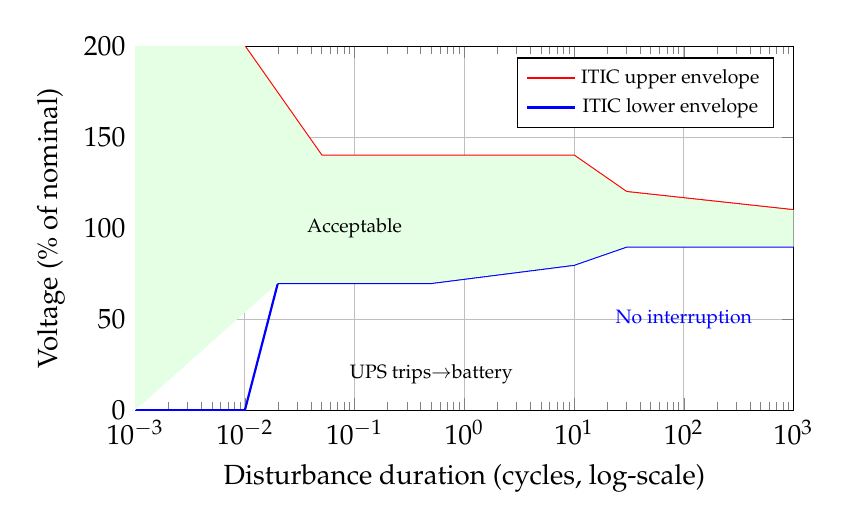
\begin{tikzpicture}
\begin{semilogxaxis}[
  width=0.82\linewidth, height=6.2cm,
  xlabel={Disturbance duration (cycles, log-scale)},
  ylabel={Voltage (\%\ of nominal)},
  xmin=0.001, xmax=1000, ymin=0, ymax=200,
  grid=major,
  legend pos=north east,
  legend style={font=\scriptsize},
  log basis x=10,
]
% Upper envelope (overvoltage tolerance)
\addplot[red,thick] coordinates {
  (0.001,500) (0.01,200) (0.05,140) (0.5,140)
  (10,140) (30,120) (1000,110) };
\addlegendentry{ITIC upper envelope}

% Lower envelope (undervoltage tolerance)
\addplot[blue,thick] coordinates {
  (0.001,0) (0.01,0) (0.02,70) (0.5,70)
  (10,80)  (30,90)  (1000,90) };
\addlegendentry{ITIC lower envelope}

% Acceptable region shading
\addplot[fill=green!10,draw=none,forget plot] coordinates
  { (0.02,70) (0.5,70) (10,80) (30,90) (1000,90) (1000,110)
    (30,120) (10,140) (0.5,140) (0.05,140) (0.01,200) (0.001,500)
    (0.001,0) (0.02,70) };

% Annotations
\node[font=\scriptsize] at (axis cs:0.1,100) {Acceptable};
\node[font=\scriptsize,red] at (axis cs:0.005,300) {No damage};
\node[font=\scriptsize,blue] at (axis cs:100,50) {No interruption};
\node[font=\scriptsize] at (axis cs:0.5,20)  {UPS trips$\to$battery};
\end{semilogxaxis}
\end{tikzpicture}
\caption{Stylised ITIC/CBEMA voltage tolerance envelope. The
green band is the safe operating region for sensitive IT equipment.
Excursions below the lower (blue) curve cause the UPS to drop the
load to battery; excursions above the upper (red) curve risk
damage to power supply units. The horizontal axis is logarithmic in
cycles at \SI{50}{\hertz}/\SI{60}{\hertz}, spanning roughly half a
microsecond to 20 seconds.}
\label{fig:itic}
\end{figure}

\subsection{Generator transient response and the ATS transfer window}\label{ss:atw}

When utility power fails, the Automatic Transfer Switch (ATS) signals
the standby generator to start. The diesel/gas engine accelerates,
the alternator field is excited, and once voltage and frequency are
within tolerance the ATS closes onto the generator. The full
sequence takes 8--12 seconds, but the most violent part is the
\emph{first cycle} of loading.

The generator's transient response when loaded is governed by its
sub-transient reactance $X_d''$, transient reactance $X_d'$, and
synchronous reactance $X_d$:
\begin{equation}\label{eq:Igen}
   I(t) \;=\; E_f \left[
   \frac{1}{X_d} + \left(\frac{1}{X_d'}-\frac{1}{X_d}\right)e^{-t/T_d'}
            + \left(\frac{1}{X_d''}-\frac{1}{X_d'}\right)e^{-t/T_d''}\,\right],
\end{equation}
where $T_d', T_d''$ are the corresponding time constants
(seconds, milliseconds respectively) and $E_f$ is field voltage.
Equation~\eqref{eq:Igen} explains why the load step that the generator
sees in its first second is several times the steady-state current:
the sub-transient reactance is much smaller than the synchronous, so
the initial current spike is large. Conservative generator sizing
($\geq 125\%$ of nominal IT load) is a direct response to this transient.

\subsection{Earthing scheme and fault propagation}\label{ss:earth}

The way the neutral is referenced to earth determines how a phase-to-earth
fault behaves --- whether it appears as a small leakage current that an
RCD detects, or as a near-bolted-fault that triggers main breaker action.

Three schemes are common:
\begin{itemize}[leftmargin=*,nosep]
  \item \textbf{TN-S} (separate neutral and protective earth):
        first phase-to-earth fault is a full short circuit, cleared by
        the breaker. Dominant in IT/PDU layers because it gives
        predictable short-circuit currents.
  \item \textbf{TN-C-S}: combined upstream, separated downstream;
        good cost-performance tradeoff but vulnerable to PEN-conductor breaks.
  \item \textbf{IT} (isolated neutral): first earth fault gives only a
        small displacement current; the second fault, on a different
        phase, becomes a phase-to-phase short. Used in some EU sites
        for continuity-of-service but requires insulation monitoring.
\end{itemize}
The choice affects how the elementary events $E_\bullet$ in the
fault tree~\eqref{eq:topdown} compose: in an IT scheme, the first-fault
event is harmless but the second-fault event is large; the joint
distribution is therefore highly non-Markovian and an additional state
must be added to the chain of Figure~\ref{fig:markov}.

\subsection{Putting the physics back into the hazard}\label{ss:closure}

We can now interpret each term of the hazard rate
\eqref{eq:hazard} in physical units:
\begin{equation*}
   \lambda_t \;=\; \lambda_0\, e^{-E_a/k_B T_t}
              \cdot \bigl(V_t/V_{\mathrm{nom}}\bigr)^{-\gamma_V}
              \cdot \exp(\beta_C C_t).
\end{equation*}
\begin{itemize}[leftmargin=*,nosep]
  \item $\lambda_0$ has dimensions of $\mathrm{events}/\mathrm{year}$,
        and is obtained from the steady-state Markov-chain analysis
        of \S\ref{ss:markov} together with the Th\'evenin/short-circuit
        analysis of \S\ref{ss:fault}.
  \item $E_a$ is the AIPL activation energy of the insulation system
        (transformer paper, capacitor dielectrics), \SI{0.6}{}--\SI{0.9}{\electronvolt}.
  \item $\gamma_V$ is the inverse-power-law voltage stress exponent
        from~\eqref{eq:AIPL}, calibrated from THD measurements
        \eqref{eq:THD} and dielectric endurance tests.
  \item $\beta_C C_t$ is the cyber-load Esscher tilt, with $C_t$
        in standardised log-rate units.
\end{itemize}
The deterministic grace period~\eqref{eq:tcrit} contains $UA$ and
$mc_p$, which an EE/HVAC engineer measures directly during
commissioning. \emph{This is the closure of the loop}: every parameter
in the actuarial pricing equation has a physical measurement
attached, and the parameters are identified, not assumed.


% ============================================================
\begin{thebibliography}{99}\small
\bibitem[Balkema and de~Haan(1974)]{Balkema1974}
A.~A. Balkema and L.~de~Haan, ``Residual life time at great age,''
\textit{Ann. Probab.}, vol.~2, pp.~792--804, 1974.

\bibitem[Black(1969)]{Black1969}
J.~R. Black, ``Electromigration --- a brief survey and some recent
results,'' \textit{IEEE Trans. Electron Dev.}, vol.~ED-16,
pp.~338--347, 1969.

\bibitem[Baldwin Group(2025)]{Baldwin2025}
The Baldwin Group, ``Data centers: risk and insurance across the
development lifecycle,'' January 2026.

\bibitem[Chhikara and Folks(1989)]{Chhikara1989}
R.~S. Chhikara and J.~L. Folks, \textit{The Inverse Gaussian
Distribution: Theory, Methodology, and Applications}, Marcel Dekker,
1989.

\bibitem[CyberCube(2025)]{CyberCube2025}
CyberCube, ``AWS US-East-1 Security Incident Report,''
preliminary loss range \$38--581\,M, October 2025.

\bibitem[Engineering News-Record(2025)]{ENR2025}
P.~Sisson, ``Report: Billions of dollars in data center construction
risk is uninsured,'' \textit{Engineering News-Record}, 2025.

\bibitem[NIRS(2025)]{NIRS2025}
Uptime Institute Intelligence, ``South Korean data center fire sparks
a stark reminder,'' November 2025.

\bibitem[NetworkWorld(2023)]{NetworkWorld2023}
A.~Bednarz, ``Data center fires raise concerns about lithium-ion
batteries,'' \textit{NetworkWorld}, March 2023.

\bibitem[Parametrix(2022)]{Parametrix2022}
M.~Lebovits, ``Insuring the cloud,'' American Academy of Actuaries,
September 2022.

\bibitem[Pickands(1975)]{Pickands1975}
J.~Pickands, ``Statistical inference using extreme order statistics,''
\textit{Ann. Statist.}, vol.~3, pp.~119--131, 1975.

\bibitem[Stull(2011)]{Stull2011}
R.~Stull, ``Wet-bulb temperature from relative humidity and air temperature,''
\textit{J. Appl. Meteorol. Climatol.}, vol.~50, pp.~2267--2269, 2011.

\bibitem[Trivedi(2017)]{Trivedi2017}
K.~S. Trivedi, \textit{Probability and Statistics with Reliability,
Queuing and Computer Science Applications}, 2nd ed., Wiley, 2017.

\bibitem[Uptime Institute(2024)]{Uptime2024}
Uptime Institute, ``Annual Outage Analysis 2024.''

\bibitem[Wang(2000)]{Wang2000}
S.~S. Wang, ``A class of distortion operators for pricing financial
and insurance risks,'' \textit{J. Risk Insur.}, vol.~67,
pp.~15--36, 2000.
\end{thebibliography}

\end{document}
